% Chapter 1

\chapter{Neutron Measurements at IP2I cryogenic facility} % Main chapter title

\label{ChapterNeutron} % Change X to a consecutive number; for referencing this chapter elsewhere, use \ref{ChapterX}

%----------------------------------------------------------------------------------------
%	BEGING CHAPTER
%----------------------------------------------------------------------------------------


\section{Motivation}

The \Ricochet{} experiment is based on the operation of cryogenic bolometers with an intense neutrino flux. This flux is produced by the ILL research nuclear reactor. The \Ricochet{} experimental setup will be located at a few meters of the reactor. As such, there is a risk that the bolometers will be blinded by the radioactive background of the ILL site, produces electronic recoils and nuclear recoils. 
The electronic recoils are mainly produced by gamma rays and charged particles such as electrons and muons. These recoils are easily discarded from the neutrino-nucleon elastic recoils thanks to the discrimination provided by the double energy measurement (ionization and heat) of the detectors.
The nuclear recoils are induced by neutrons. This neutron background generates the same signal as the CENNS and as such cannot be readily discriminated by the detector. It is an unavoidable background for \Ricochet{} which will limit the CENNS process measurement.
Nevertheless, it is possible to achieve a likelihood analysis with an estimation of the nuclear recoil rate produced by the neutron background. This background-induced component can be deducted from the total nuclear recoil spectrum to evaluate the spectrum generated by neutrino-nucleon scattering. 
Therefore, it is vital to evaluate the neutron background on-site and understand its dependency in the energy.
In addition to estimating the limitations on the measurement, the study of the neutron background on-site will also be used in the design of the shielding.

With the current experimental setup, it is not possible to measure the ILL neutron background in the energy range of the detectors. 
%Such techniques for the neutron background measurement are presented in the latter paragraph \ref{par:perspectives} assessing the perspectives of the \Ricochet{} experiment in regards to the neutron background measurement.
For now, the neutron background is extrapolated from its measurement at higher energy range.
The neutron energy spectrum is measured at the ILL site with gaseous Helium-3 Tube Detector based on the neutron capture by \ce{^3He}:
\begin{equation}
	\ce{^1_0n + ^3_2He -> ^3_1H + ^1_1p}
\end{equation}
This spectroscopy approach is sensitive to fast neutrons of energy $\mathcal{O}(\SI{1}{\mega\eV})$. As these fast neutrons produce \si{\kilo\eV}-scale nuclear recoils in germanium detectors via elastic scattering suggesting that a \ce{^3He} fast neutron measurement will allow us to anticipate the fast neutron background for \Ricochet{}.
This chapter is focused on the measurement of fast neutrons at IP2I achieved with the cryogenic germanium detectors and its corresponding data analysis.


\section{Experimental Setup}

The reference neutron background is measured at the IP2I cryostat facility. 
%The measurement at high energy range $\mathcal{O}(\SI{1}{\mega\eV})$ is achieved with a \ce{^3He} tube detector while the measurement at low energy range $\mathcal{O}(\SI{10}{\kilo\eV})$ is assured by the cryogenic detector RED80.
The figure \ref{fig:scheme-ip2i} presents on the right a scheme of the cryostat facility with the position of the detectors. RED80 is operated inside the cryostat. The \ce{^3He} tube detector is operated inside the disassembled cryostat while keeping the same distance to the neutron source. The measurements are separated in two phases: the neutron Calibration and the Background measurement.

During the neutron Calibration phase, the detectors measure a lot of nuclear recoils as to calibrate the analysis yielding the energy spectrum. A neutron source is used to generate these nuclear recoils in the detectors. The figure \ref{fig:scheme-ip2i} displays on the left a photo of the neutron source setup used for the measurement. It consists in the AmBe neutron source, already use for the neutron activation of the germanium described in paragraph \ref{par:calibration-sources}, surrounded by milk bricks and a lead brick wall. The milk bricks create an efficient low-cost water shielding as to thermalize the neutrons. The lead brick wall is positioned between the neutron source and the detectors. Its role is to stop the gamma rays produced by the neutron source and assure a stable radioactive electronic background for the detectors.
In this phase, the neutron source is placed at the position $C$, approximately \SI{2.5}{\meter} from the center of the cryostat. This position was found empirically to be close enough to provide an intense neutron flux without saturating the detectors.

During the Background measurement phase, the detectors are isolated from the neutron source as to measure nuclear recoils produced solely by the neutron background of the IP2I facility. The source is placed in its storage in position $B$ more than \SI{10}{\m} away from the cryostat.
%This position was confirmed to be safe for the isolation of the detector with a comparison measurement with the neutron source outside of the laboratory.

\begin{figure}
\centering
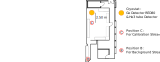
\includegraphics[scale=1]{Figures/Neutron/neutron_source_ip2i.pdf}
\caption{On the left, photo of the neutron source used for the Calibration streams in position $C$. It consists in the AmBe neutron source surrounded by milk bricks and a lead brick wall on the cryostat-facing side. On the right, overhead view scheme of the IP2I cryostat facility for the neutron background measurements. The \ce{^3He} tube detector and RED80 are located on the cryostat. The neutron source can be in position "C"  near the detectors for neutron Calibration streams and in position "B" away for the Background streams.}
\label{fig:scheme-ip2i}
\end{figure}

In section \ref{par:ill-neutron-background}, we compare the \ce{^3He} capture rate with the nuclear recoil detection rate in cryogenic germanium detectors.

The low energy measurements with RED80 were carried out during the run 57. This run started on 03/07/2019 and ended on 01/08/2019. The detector RED80 was operated in the suspended tower of the cryostat along with the detector RED70 (not studied in this work). The detector RED80 is fully described in the previous chapter \ref{ChapterElectrodesExperimental} using several streams of the run 57.

Before being installed into the cryostat, the germanium crystal of RED80 was activated with an AmBe neutron source as described in section \ref{par:calibration-sources}. As such, the detector possesses two intrinsic and uniformly distributed calibration peaks of electronic recoils at \SI{1.3}{\kilo\eV} and \SI{10.37}{\kilo\eV}. The neutron activation started on 28/06/2019 at 17h08 and ended on 02/07/2019 at 10h08 yielding \SI{89}{\hour} of activation.

% Conditions of data taking
Several data streams are attributed to the IP2I neutron background measurement. The table \ref{tab:neutron-streams} lists the data streams and their starting date. Depending on the position of the neutron source, the streams are attributed to the Background phase or the Calibration phase.
Each stream was taken during nights or week-ends to benefit from long time of stable operation. The configurations were mixed in term of dates. This is of importance when measuring the rate of the calibration peak electronic recoils which is decreasing with time as discussed in section \ref{par:calibration-sources}.

In all the streams, RED80 was operated at \SI{16}{\milli\kelvin} with an optimal NTD polarization current of \SI{1}{\nano\ampere}. The electrodes were polarized in their default configuration (eq. \ref{eq:red80-default-polarization}) with a voltage bias $V_{bias} = \SI{2}{\volt}$.

\begin{table}[]
\centering
\begin{tabular}{l|c|c|c|c}
Configuration                & Stream   & Starting Date & Stream Duration / \si{ \hour} & Cumulative Duration / \si{ \hour}  \\ \hline \hline
\multirow{3}{*}{Background}  & tg18l005 & 18/07/2019  & 14.95 & \multirow{3}{*}{52.88}\\
                             & tg27l000 & 27/07/2019 & 16.43 & \\
                             & tg28l000 & 28/07/2019 & 21.50 & \\ \hline
\multirow{4}{*}{Calibration} & tg17l007 & 17/07/2019 & 11.83 & \multirow{4}{*}{75.99} \\
                             & tg19l010 & 19/07/2019 & 20.86 &\\
                             & tg20l000 & 20/07/2019 & 26.37  & \\
                             & tg21l000 & 21/07/2019 & 16.93  &
\end{tabular}
\caption{Starting data and duration of the data streams attributed to the IP2I neutron background measurement. For the Calibration configuration, the neutron source is facing the cryostat in position $C$. For the Background configuration, the detector is isolated from the neutron source stored in position $B$. The cumulative duration of each configuration is calculated.}
\label{tab:neutron-streams}
\end{table}


\section{Analysis of the Data Streams}
\label{par:analysis-data-streams}

The data streams are pre-processed with the NEPAL software as discussed in section \ref{par:analysis-pipeline}. The majority of the analysis steps are already described in the chapter \ref{ChapterElectrodesExperimental}. 
In this section, analysis steps specific to the neutron measurements and differences in the cut parametrization are presented. The figure \ref{fig:cut-venn-diagramm} summarizes the event types depending on their passing cuts.
Compared to the characterization study of RED80 and REDN1 presented in the previous chapter \ref{ChapterElectrodesExperimental}, the stream used for the IP2I neutron background measurement are long and yield plenty of statistics. As such, the analysis cuts are globally more conservative with smaller tolerances compared to previous studies. 

%The section starts with the description of an additional analysis step, the "live time cut". Then, it presents and justifies the quality cut parametrization. Later, it introduces a cut on the charge conservation

\begin{figure}
\centering
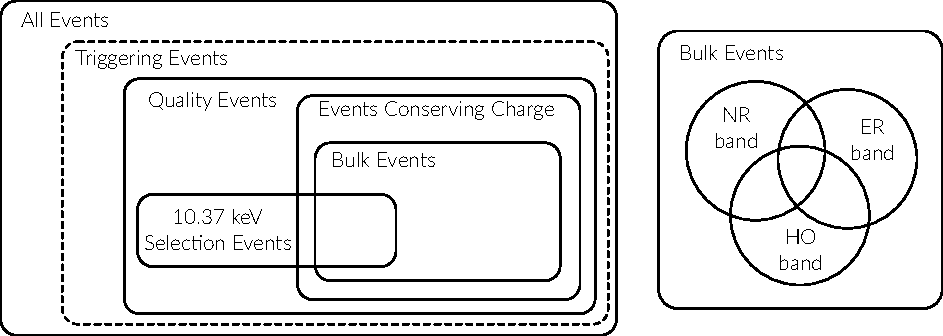
\includegraphics[scale=1]{Figures/Neutron/cut_venn_diagramm.pdf}
\caption{Venn diagrams of the events in the presented analysis for the measurement of the neutron background. The dashed class "Triggering Events" is only used for the events generated by the pulse simulation.}
\label{fig:cut-venn-diagramm}
\end{figure}


\subsection{Parametrization of the Quality Cuts}
\label{par:param-quality-cuts}

The quality cuts are described in the dedicated section \ref{par:quality-cuts}. For this analysis, the maintenance cut, the reset cut and the ionization offset cut are applied with the same parametrization.
The live time cut and the $\chi^2$ cut are applied with specific parameters. 

The table \ref{tab:live-time-cut} lists the selected time intervals for each stream in regards to the live time cut. Even though the data streams were recorded for long and apparently stable operation, some portion of the streams were corrupted. As the exact causes are unknown at this time, the intervals were chosen with some precautionary buffer as to only record data during stable electronics operation.
The live time cut is used to evaluate the cumulative live time $T_{live}$ for each configuration. These are used later in section \ref{par:normalization} in the calculation of the detector exposure.

\begin{table}[]
\centering
\begin{tabular}{l|l|c|c}
Configuration & Stream & Selected Intervals / \si{\hour} & $T_{live}$ \\ \hline \hline
\multirow{3}{*}{Background}  & tg18l005 & $[0, 7.4] \cup [7.6, 14.95]$& \multirow{3}{*}{ $\SI{35.93}{\hour} = \SI{1.497}{\day}$ }  \\
                             & tg27l000 & $[0, 7] \cup [11.3, 13.8] \cup [14.1, 16.43]$ &                        \\
                             & tg28l000 & $[0, 7.4] \cup [8.05, 10]$ &                        \\ \hline
\multirow{4}{*}{Calibration} & tg17l007 & $[0, 11.83]$ & \multirow{4}{*}{ $\SI{75.60}{\hour} = \SI{3.150}{\day}$ } \\
                             & tg19l010 & $[0, 8.30] \cup [8.70, 11.83]$ &                        \\
                             & tg20l000 & $[0, 26.73]$ &                        \\
                             & tg21l000 & $[0, 16.93]$ &                       
\end{tabular}%
\caption{Selected time intervals for live time cut of each stream. The cumulative live time $T_{live}$ is evaluated for the Background and Calibration configurations.}
\label{tab:live-time-cut}
\label{tab:neutron-live-time}
\end{table}

The table \ref{tab:neutron-quality-cuts} lists the parameters used for the $\chi^2$ cuts for each stream of the analysis. The three parameters $\chi_0^2$, $A_0$ and $b$ corresponds to the $\chi^2$ threshold function defined in equation \ref{eq:chi2-threshold-function}.

\begin{table}[]
\centering
\begin{tabular}{c|l|l|c|c|c}
Configuration & Channel & Stream   & $\chi_0^2$                                & $A_0$ & $b$ \\ \hline \hline
\multirow{8}{*}{\begin{tabular}[c]{@{}c@{}}Background\\ \&\\ Calibration\end{tabular}} &
  \multirow{7}{*}{Heat} &
  tg17l007 &
  \multirow{5}{*}{400} &
  \multirow{7}{*}{\num{3e2}} &
  \multirow{7}{*}{2} \\
              &         & tg18l005 &                                           &       &     \\
              &         & tg19l010 &                                           &       &     \\
              &         & tg20l000 &                                           &       &     \\
              &         & tg21l000 &                                           &       &     \\ \cline{3-4}
              &         & tg27l000 & \multicolumn{1}{l|}{\multirow{2}{*}{700}} &       &     \\
              &         & tg28l000 & \multicolumn{1}{l|}{}                     &       &     \\ \cline{2-6} 
 &
  \begin{tabular}[c]{@{}l@{}}Ionization\\ $A,B,C,D$\end{tabular} &
  All &
  \multicolumn{1}{r|}{300} &
  \multicolumn{1}{r|}{\num{2e3}} &
  \multicolumn{1}{r}{2.2}
\end{tabular}
\caption{Parameters for the quality cuts used in the Neutron Analysis.}
\label{tab:neutron-quality-cuts}
\end{table}


\subsection{Cross-talk Correction and Calibration}

The analysis steps following the application of the quality cuts are the cross-talk correction, the selection of the \SI{10.37}{\kilo\eV} calibration peak events and the calibration of the heat and ionization channels. These steps are described in the section \ref{par:analysis-pipeline}.

The cross-talk correction relies on the estimation of the capacitance of the cabling. For RED80 in the run 57, this capacitance was already evaluated to  $C_{cabling} = \SI{125}{\pico\farad}$. Repeating this estimation with the streams yield values within the error bars. As such, this cabling capacitance is conserved for this analysis.

For the measurement of the IP2I neutron background, the selection of the \SI{10.37}{\kilo\eV} calibration peak events  is solely used for the calibration of the heat and ionization channels.
In the case of Background streams, the selection and calibration are the same as for the previous study of RED80.
In the case of Calibration streams, this selection is hampered by the highly populated nuclear band. The selection of the \SI{10.37}{\kilo\eV} calibration events described in section \ref{par:10kev-selection} is contaminated with events from the continuous nuclear recoil band. A s such, the calibration of the heat channel is realized with the events above the nuclear recoil band only. There is almost no loss of precision on the estimation of the calibration peak and on the calibration coefficient $\alpha_{heat}$ of equation \ref{eq:calibration-heat}. 
%However, the verification of the Luke-Neganov effect have more uncertainty, which is of minor concern.


\subsection{Charge conservation cut and Parametrization of the Bulk Cut}
%\label{par:charge-conservation-cut}
%\label{par:param-bulk-cut}

The electric charge conservation was already discussed for the characterization study of RED80 and REDN1 in the section \ref{par:charge-conservation-cut}. There was no clear evidence that a population of events not conserving the electric charge does exist. 
The charge conservation cut is applied with the same parametrization: events passing this cut have a charge conservation energy $E_{CC}$ inferior to 2 times the associated resolution $\sigma(E_{CC})$ (see equation \ref{eq:charge-conservation-cut}).

%The baseline resolution $\sigma_{E_{CC}}(\SI{0}{\kilo\eV_{ee}})$ is obtained from noise events as explained in the section \ref{ref:data}. The resolution $\sigma_{E_{CC}}(\SI{10.37}{\kilo\eV_{ee}})$ is computed from the selection of the \SI{10.37}{\kilo\eV} calibration events.

The bulk cut was introduced in section \ref{par:bulk-cut} also for the characterization of the RED80 and REDN1 detectors. For this analysis dedicated to the measurement of the neutron background, the tolerance on the ionization energies of the guard electrodes $E_A$ and $E_C$ are lower, now corresponding to $2 \cdot \sigma_{E_{X}}$. Thus, for this analysis, bulk events satisfy the following inequalities:
\begin{equation}
\begin{cases}
E_A < 2 \cdot \sigma_{E_A} \left( \SI{0}{\kilo\eV} \right) \\
E_C < 2 \cdot \sigma_{E_C} \left( \SI{0}{\kilo\eV} \right) 
\end{cases}
\end{equation}

For bulk events, it is more advantageous to use the bulk ionization energy $E_{Ion.}^{bulk}$ rather than the total ionization energy $E_{Ion.}^{total}$. Indeed, the bulk ionization energy is only calculated from the signal on the two main collecting electrodes $B$ and $D$ such that:
\begin{equation}
E_{Ion.}^{bulk} = \frac{E_B + E_D}{2}
\end{equation}
As a result, the standard deviation associated is lower than for the $E_{Ion.}^{total}$:
\begin{equation}
\sigma_{E_{Ion.}^{bulk}} = \sqrt{ \sigma_{E_B}^2 + \sigma_{E_D}^2  }
\simeq \frac{\sigma_{E_B}}{\sqrt{2}}
\approx \frac{\SI{260}{\eV}}{\sqrt{2}}
= \SI{183}{\eV}
\end{equation}

For the rest of the analysis, the ionization energy of the bulk events are therefore estimated with the quantity $E_{Ion.}^{bulk}$. In particular, this propagates to the calculation of the recoil energy $E_R$ and the quenching factor $Q$.


\subsection{Comparison of the Calibration and Background Data}
\label{par:comparison-background-calibration}

Up until now, the analysis was focused on pruning events with possibly bad energy reconstruction energy and calibrating the heat and ionization channel. All the previous analysis steps, summarized on the left of scheme \ref{fig:cut-venn-diagramm}, yields the bulk events. These events, being from Calibration or Background streams, passed the quality cuts, the charge conservation cut and the bulk cut.
Each bulk event is now characterized by two quantities: its heat energy $E_{heat}$ expressed in \si{\kilo\eV_{ee}} and its bulk ionization energy 
$E_{Ion.}^{bulk}$ in \si{\kilo\eV}.
These two quantities can be converted into the recoil energy $E_R$ in \si{\kilo\eV} and the quenching factor $Q$ according to the following equations:
\begin{align}
\label{eq:er-quenching}
E_R 
&= 
E_{heat}
\cdot
\left( 1 + \frac{V_{bias}}{\epsilon_{e^--h^+}} \right) - E_{Ion.}^{bulk} \frac{V_{bias}}{\epsilon_{e^--h^+}}
\\
Q &= \frac{E_{Ion.}^{bulk}}{E_R}
\end{align}
with $V_{bias}=\SI{2}{\volt}$ the voltage bias of RED80 of use for the Luke-Neganov effect calculation (see equation \ref{eq:luke-neganov-energy}) and $\epsilon_{e^--h^+}=\SI{2.97}{\eV}$ the average energy of an electron-hole pairs.
The quenching factor $Q$ is useful to illustrate the discrimination between the electronic and the nuclear recoils in the germanium. As for the recoil energy $E_R$, it corresponds to the total energy that is transferred to the crystal through the particle interaction with the crystal.

The top graphic of the figure \ref{fig:ecei-quenching-annotation} is a scatter plot of the bulk ionization energy $E_{Ion.}^{bulk}$ versus the heat energy $E_{heat}$ for all the bulk events used in this analysis. The bottom plot represents the quenching $Q$ versus the recoil energy $E_R$ of the bulk events. In both plots, the events originating from the Calibration and Background streams are colored blue and black respectively. The numbers $1$ to $6$ annotates different event types.

\begin{figure}
\centering
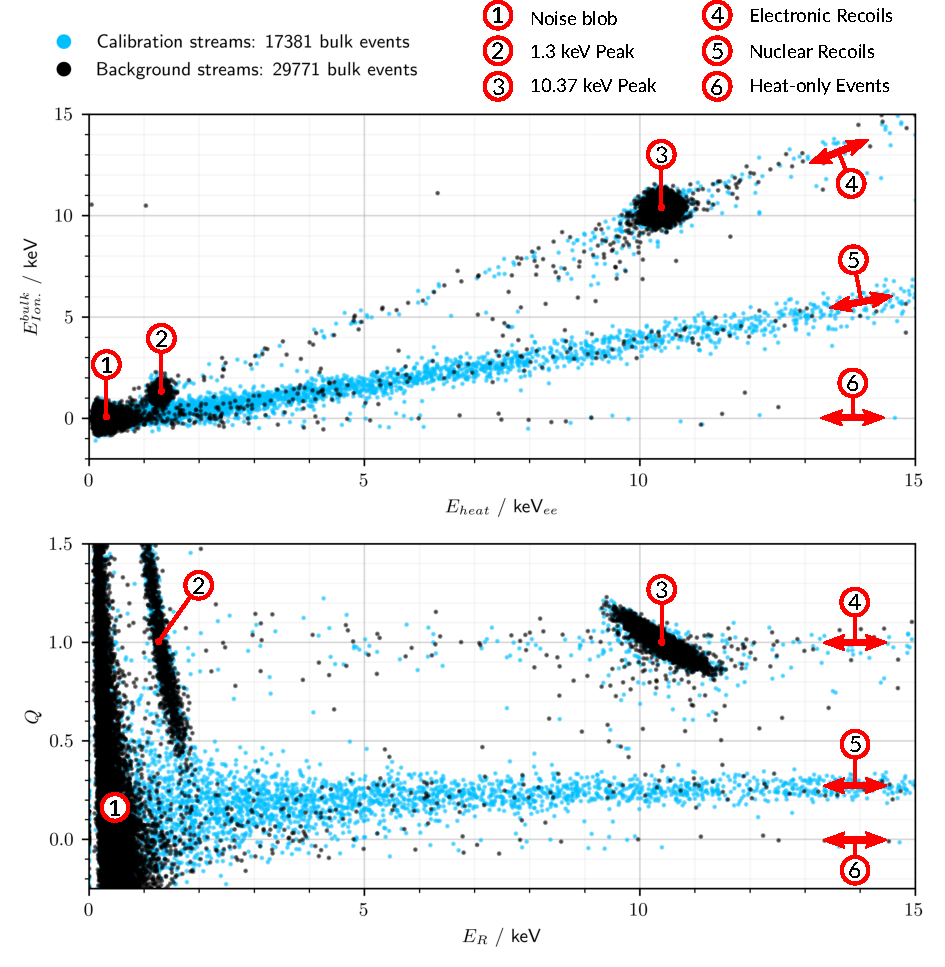
\includegraphics[width=\linewidth,]{Figures/Neutron/ecei_quenching_annotation.pdf}
\caption{At the top, bulk ionization energy $E_{Ion.}^{bulk}$ of all bulk events versus their heat energy $E_{heat}$. At the bottom, quenching $Q$ of all the bulk events versus their recoil energy $E_R$. Events from Calibration streams are in blue. Events from the Background streams are in black.}
\label{fig:ecei-quenching-annotation}
\end{figure}

%% noise blob
The noise blob, labeled $1$, corresponds to triggering noise windows and with events of very low energy. It is a feature common to all the streams.
%As a result, the position of the noise blob is centered on the triggering threshold of the heat channel
The position of the noise blob is the origin:
\begin{equation}
\begin{cases}
E_{Ion.}^{bulk} = \SI{0}{\kilo\eV} \\
E_{heat} = \SI{0}{\kilo\eV}_{ee}
\end{cases}
\end{equation}
As a result, it is next-to impossible to evaluate the quenching of the events. This explains the shape of the noise blob in the $Q$ vs $E_R$ bottom plot. It covers the entire range of the quenching value with the merging of the electronic, nuclear and heat-only bands.

% 1.3 kev calibration peak
The population labeled $2$ corresponds to the \SI{1.3}{\kilo\eV} calibration peak. This population is present in both the Calibration and Background streams. These events are induced by electronic recoils, thus belongs to the electronic recoil band, and are characterized by the following quantities:
\begin{equation}
\textsf{\SI{1.3}{\kilo\eV} line:}
\begin{cases}
E_{Ion.}^{bulk} = \SI{1.3}{\kilo\eV} \\
E_{heat} = \SI{1.3}{\kilo\eV}_{ee} \\
Q = 1 \\
E_R = \SI{1.3}{\kilo\eV}
\end{cases}
\end{equation}
The energies of these events are close to the energy resolution. Consequently, the estimation of the quenching factor $Q$ is imprecise which explains the banana shaped of the population on the $Q$ versus $E_R$ plot.

% 10.37kev calibration peak
The \SI{10.37}{\kilo\eV} calibration peak is labeled $3$. These events are present in all the streams. The population is centered on the quantities:
\begin{equation}
\textsf{\SI{10.37}{\kilo\eV} line:}
\begin{cases}
E_{Ion.}^{bulk} = \SI{10.37}{\kilo\eV} \\
E_{heat} = \SI{10.37}{\kilo\eV}_{ee} \\
Q = 1 \\
E_R = \SI{10.37}{\kilo\eV}
\end{cases}
\end{equation}
Their heat and ionization energies is high enough for a precise estimation of the quenching factor. However, the calculation of the recoil energy $E_R$ leads to a warped blob in the $Q$ versus $E_R$ plot. 
One can note a remnant of the \SI{10.37}{\kilo\eV} calibration events with incomplete charge collection as studied in section \ref{par:10kev-selection}. They consists in in the inter-band events between the ER and NR bands with incomplete charge collection.

%% ER band
The electronic recoil band, or ER band, is indicated by the number $4$. The majority of the events originating from the Background streams are in this band, indicating that the radioactive background of the IP2I cryostat facility mainly induces electronic recoils. The two calibration peaks are part of the electronic recoil band. An event of the ER band with a recoil energy $E_R$ is characterized by the following quantities:
\begin{equation}
\label{eq:er-band}
\textsf{Gamme ER band:}
\begin{cases}
Q = Q_{ER} = 1 \\
E_{Ion.}^{bulk} = Q \cdot E_R = E_R \\
E_{heat} = E_R
\end{cases}
\end{equation}

% NR band
The nuclear recoil band, or NR band, is annotated by the number $5$. This band is densely populated for the Calibration streams. This confirm that the neutron source is well placed so that the majority of the triggering events are nuclear recoils. These events are also present in the Background streams although with much less statistics. These events are characterized with:
\begin{equation}
\label{eq:nr-band}
\textsf{Neutron NR band:}
\begin{cases}
Q = Q_{NR} \left( E_R \right) \\
E_{Ion.}^{bulk} = Q_{NR}\left( E_R \right) \cdot E_R \\
E_{heat} 
=
E_R 
\cdot
\frac{
1 + Q_{NR} \left( E_R \right)\frac{V_{bias}}{\epsilon_{e^--h^+}}
}{
1 + \frac{V_{bias}}{\epsilon_{e^--h^+}}
}
\end{cases}
\end{equation}
The quenching factor $Q_{NR}$ associated with the nuclear recoils is a function of the recoil energy $E_R$.
The nuclear recoils from the Background streams are precisely what corresponds to the IP2I neutron background and consist in the intrinsic limit to the measurement of the CENNS process.

%% Heat-only events
The number $6$ indicated a much less populated band of events displaying a quenching of $Q=0$. These events are known as "Heat-only" events, HO events. This population is infamously known in all dark matter experiments (\Edelweiss{}, CDMS and CRESST) using cryogenic crystalline detectors. These events produce a signal solely on the heat channel. They are characterized by the quantities:
\begin{equation}
\label{eq:ho-band}
\textsf{Heat-only band:}
\begin{cases}
Q = Q_{HO} = 0 \\
E_{Ion.}^{bulk} = \SI{0}{\kilo\eV}\\
E_{heat} 
=
E_R 
\cdot
\frac{
1
}{
1 + \frac{V_{bias}}{\epsilon_{e^--h^+}}
}
\end{cases}
\end{equation}
They could correspond to electronic and nuclear events with no charge collection due to all charges being trapped or recombining on the electrodes, as discussed in section \ref{par:trapping}. However, this is not compatible with the lower counts of inter-band events with an incomplete charge collection. Moreover, the HO events are present in all the streams with an apparent independence from the Background and Calibration configurations, and the calibration peaks.
At this moment, their origin is unknown and is still under investigation.
%An other and more realistic explanation would be the existence of energy deposit in the crystal without ionization. 

The presence of the three ER, NR and HO bands in this plot demonstrate the discriminating ability of the double heat and ionization energy measurement. One can note that although the bands are well separated at high energy, they are merging at low energy due to their width which is fixed by the energy resolution of the heat and ionization channel. The merging phenomenon of the bands at low energy is also more visible in the bottom graph $Q$ versus $E_R$. We can even visually witness that the lower part of the \SI{1.3}{\kilo\eV} event blob is leaking into the higher part of the nuclear band.


\subsection{Band cuts and Unnormalized Energy Spectra}
\label{par:band-cut}

The objective of this analysis is to extract the energy spectrum of events associated to the nuclear recoils. In order to attribute each event to a recoil type, the so-called "Band Cuts" are defined. There are three cuts, each corresponding to the three electronic recoils, nuclear recoils and heat-only event bands. An event is attributed to a band if it is passing the associated cut. A band cut is base on the comparison between the experimental bulk ionization energy $E_{Ion.}^{bulk}$ and the theoretical ionization energy $E_{Ion.}^{theory}(band)$ expected from an event belonging to the band. This theoretical energy is calculated using the characterization of the bands introduced in the previous section \ref{par:comparison-background-calibration}. The tolerance is chosen to be two standard deviation of the bulk ionization energy $\sigma_{E_{Ion.}^{bulk}}$ at the considered heat energy $E_{heat}$. The cut are therefore expressed mathematically with the inequality:
\begin{equation}
|E_{Ion.}^{bulk} - E_{Ion.}^{theory}(band)| < 2 \cdot \sigma_{E_{Ion.}^{bulk}} \left( E_{heat}\right)
\end{equation}
One should note that the band cuts are defined using only the uncertainty on the ionization channel with the $2 \cdot \sigma_{E_{Ion.}^{bulk}}$ tolerance. Indeed, the resolution of the ionization channel is greater than the resolution of the heat channel. Thus, the analysis is simplified by assuming the measurement of the heat energy $E_{heat}$ to be error free.

The "ER band cut" selects the events attributed to the electronic recoil band. The cut parametri\-za\-tion is based on the theoretical characterization of the electronic recoils presented in the system of equations \ref{eq:er-band}. Passing events, deemed "ER events" satisfy the inequality:
\begin{equation}
\label{eq:condition-ER-ecei}
|E_{Ion.}^{bulk} - E_ {heat}| < 2 \cdot \sigma_{E_{Ion.}^{bulk}} \left( E_{heat}\right)
\end{equation}

The "NR band cut" is associated with the nuclear recoil band. Its parametrization uses the theoretical characterization of the nuclear recoils presented in the system \ref{eq:nr-band}. The quenching factor $Q_{NR}$ is evaluated with the Linhard model (eq. \ref{eq:lindhard}). Thus the "NR events" satisfies the inequality:
\begin{equation}
\label{eq:condition-NR-ecei}
|E_{Ion.}^{bulk} - Q_{NR} \left( E_{R} \right) \cdot E_{heat}| < 2 \cdot \sigma_{E_{Ion.}^{bulk}} \left( E_{heat}\right)
\end{equation}
with the recoil energy $E_R$ calculated from $E_{Ion.}^{bulk}$ and $E_{heat}$ with the equation \ref{eq:er-quenching}.

The "HO band cut" attributes events to the heat-only band. Using their characterization in the system of equations \ref{eq:ho-band}, the "HO events" passing this cut satisfies:
\begin{equation}
|E_{Ion.}^{bulk}| < 2 \cdot \sigma_{E_{Ion.}^{bulk}} \left( E_{heat}\right)
\end{equation}

The figure \ref{fig:band-cuts} illustrates the application of the band cuts on the bulk events originating from the Calibration streams. At the top are the bulk ionization energies $E_{Ion.}^{bulk}$ versus the heat energies $E_{heat}$. At the bottom is the quenching factor $Q$ versus the recoil energy $E_R$. Each band cut is represented with the tolerance of $2 \cdot \sigma_{E_{Ion.}^{bulk}} \left( E_{heat}\right)$ on the ionization  energy. Each band is centered on the line drawn by their theoretical characterization $E_{Ion.}^{theory}(band)$.
One should note that according to the expressions \ref{eq:nr-band}, there is no analytical expression of the ionization energy $E_{Ion.}^{theory}(\textsf{NR band})$ as a function of the heat energy. To bypass this issue, the ionization energy is computed over a fine array of heat energy from \SIrange{0}{50}{\kilo\eV}. Then, the plotted theoretical line is obtained by linear interpolation.

\begin{figure}
\centering
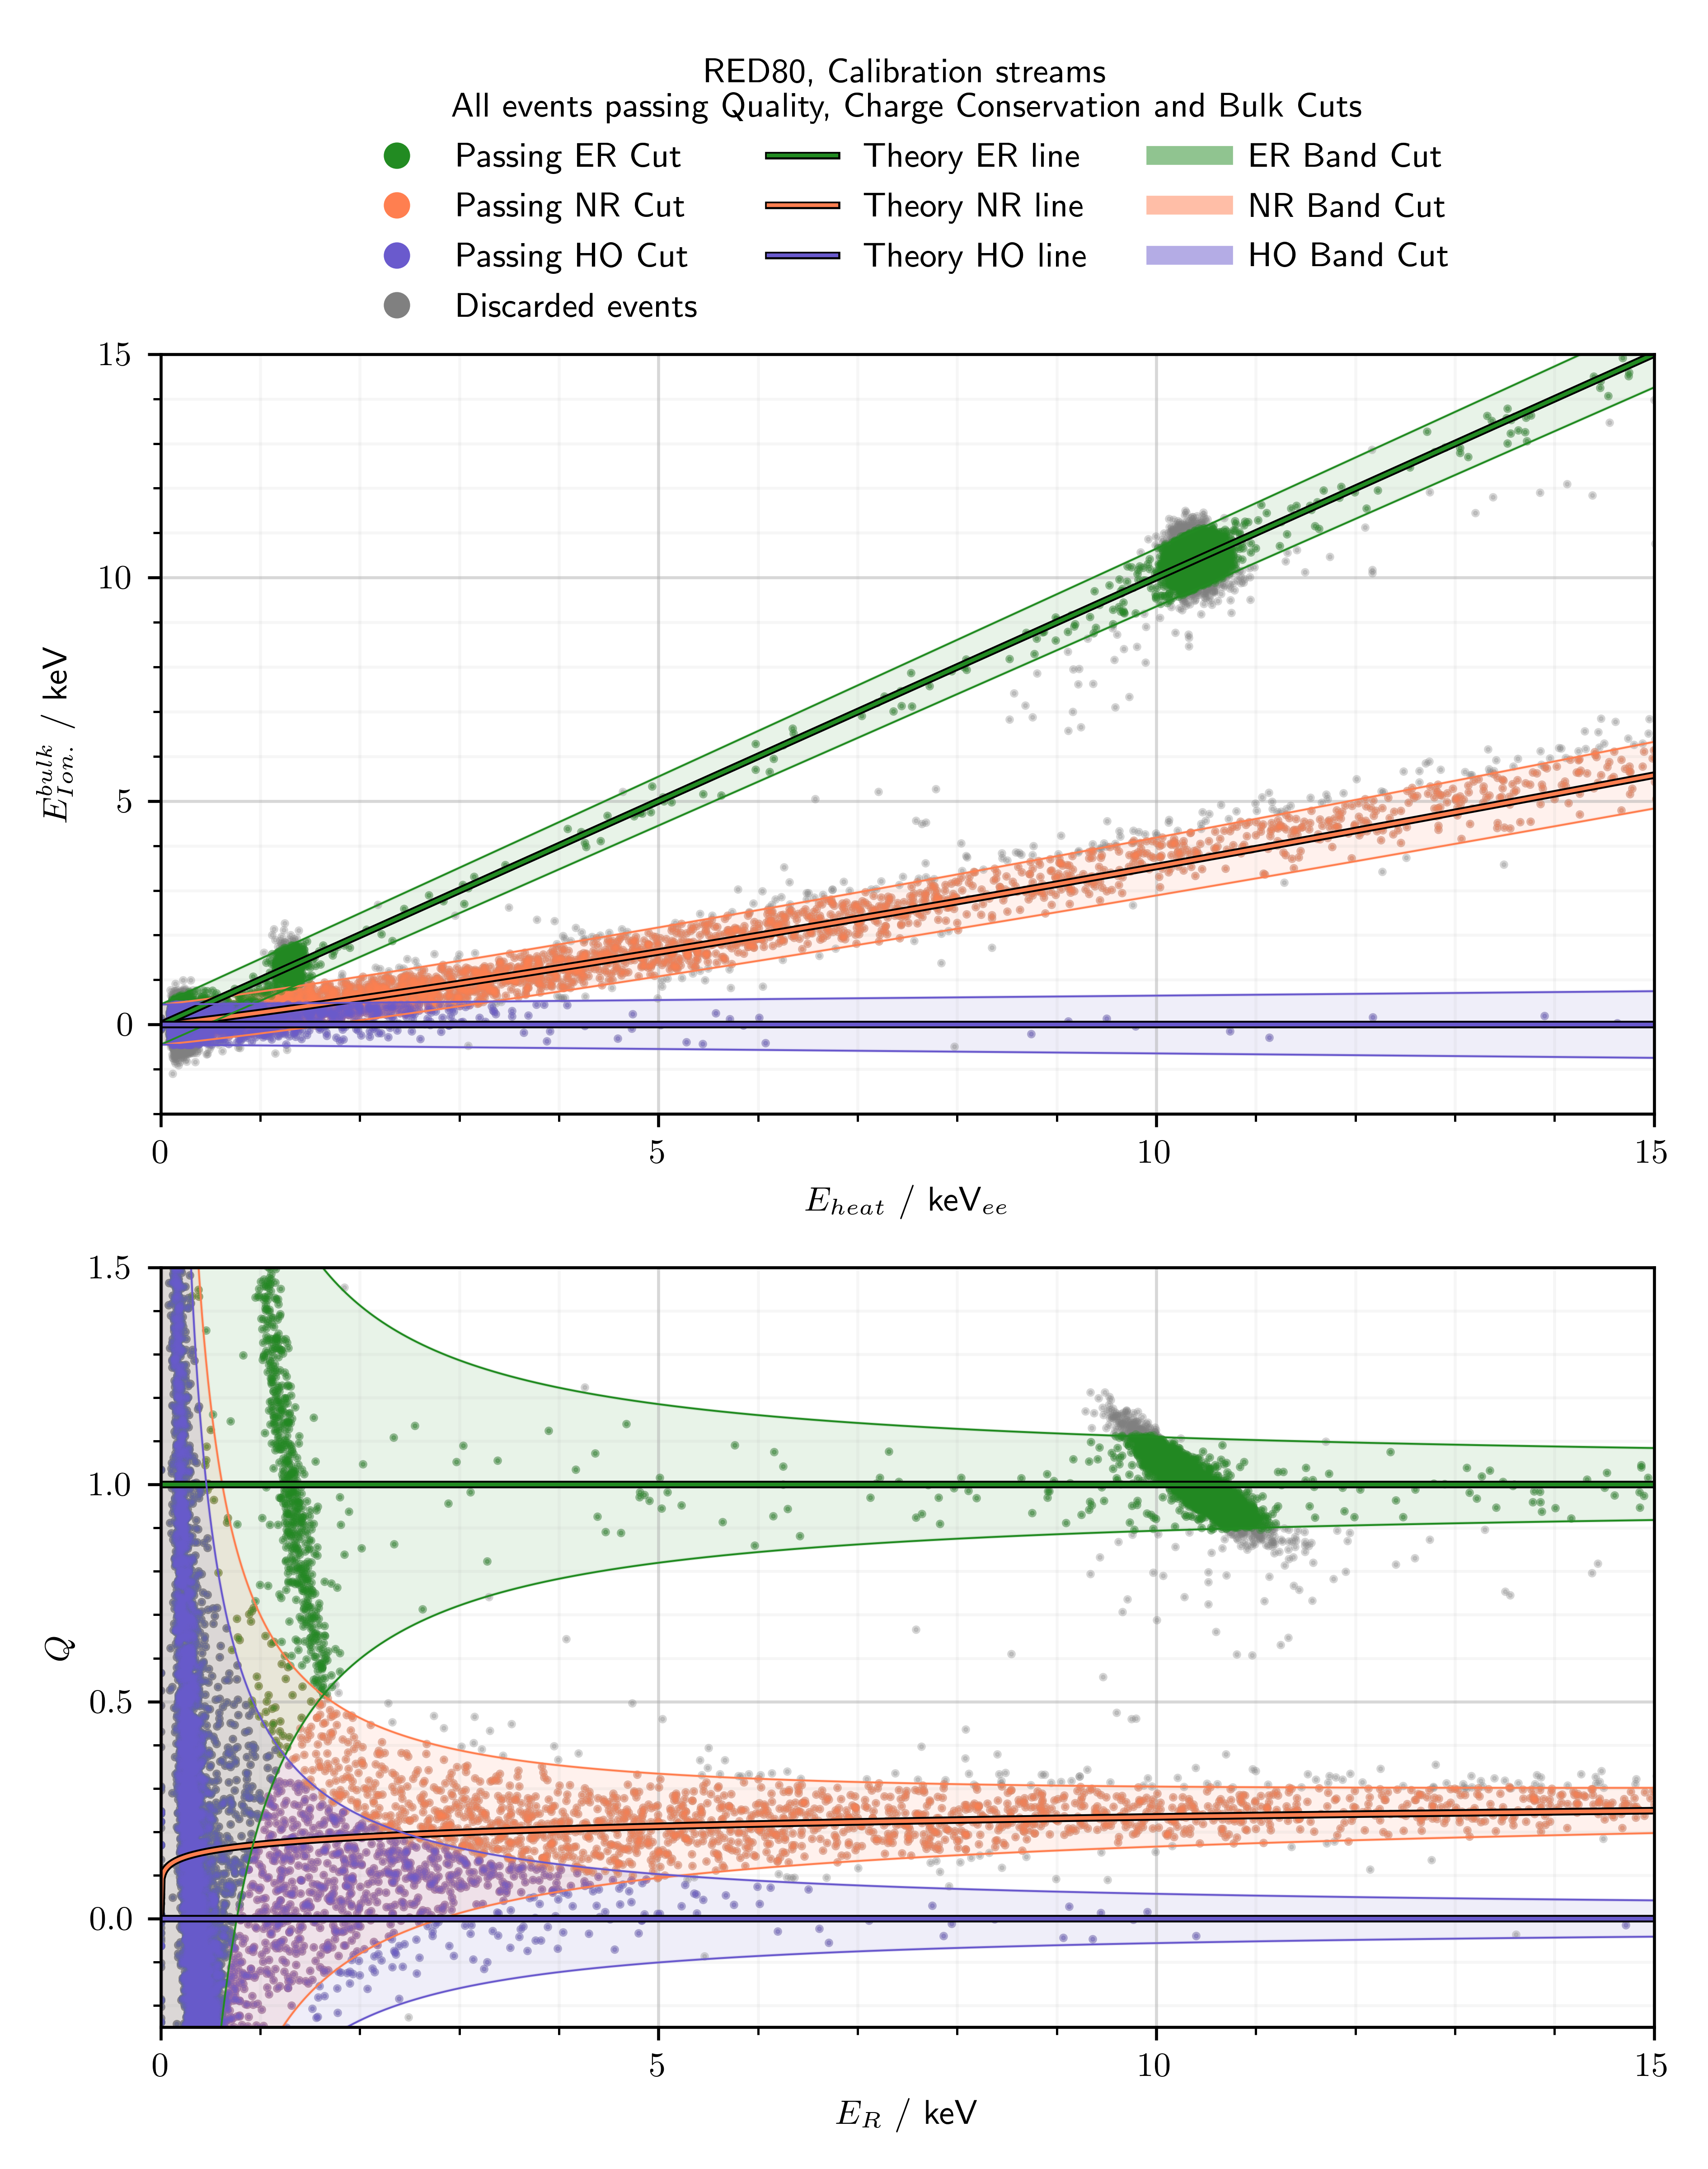
\includegraphics[scale=1]{Figures/Neutron/band_cuts.png}
\caption{Illustration of the Band cuts on the bulk events originating from the Calibration events. The top plot represents the bulk ionization energy $E_{Ion.}^{bulk}$ versus the heat energy $E_{heat}$. The bottom plot displays the quenching factor $Q$ versus the recoil energy $E_R$. The electronic recoil (ER), nuclear recoil (NR) and heat-only (HO) bands are plotted with the $2 \cdot \sigma_{E_{Ion.}^{bulk}}$ tolerance.}
\label{fig:band-cuts}
\end{figure}

We see that for $E_R \lesssim \SI{5.5}{\kilo\eV}$, the different bands are merging into each other, starting with the NR and HO bands. As bands overlap, some events are attributed to multiple bands, particularly at the lowest energies. The lower parts of the \SI{1.3}{\kilo\eV} calibration peak is even leaking into the NR band. This effect is detrimental to the counting of the number of events of each type. A compensation of this effect applied later in the analysis and is described in the dedicated section \ref{par:contamination-correction}.

At this point of the analysis, the selection of the nuclear recoils event is made with the NR band cut. A convenient review of the analysis cuts used to prune all the events is to compute the energy spectra. The figure \ref{fig:cut-histogram} displays the recoil energy $E_R$ spectra associated with the Background streams, on the top plot, and the Calibration streams, on the bottom plot. The histograms are calculated with bins of \SI{1}{\kilo\eV} width.

\begin{figure}
\centering
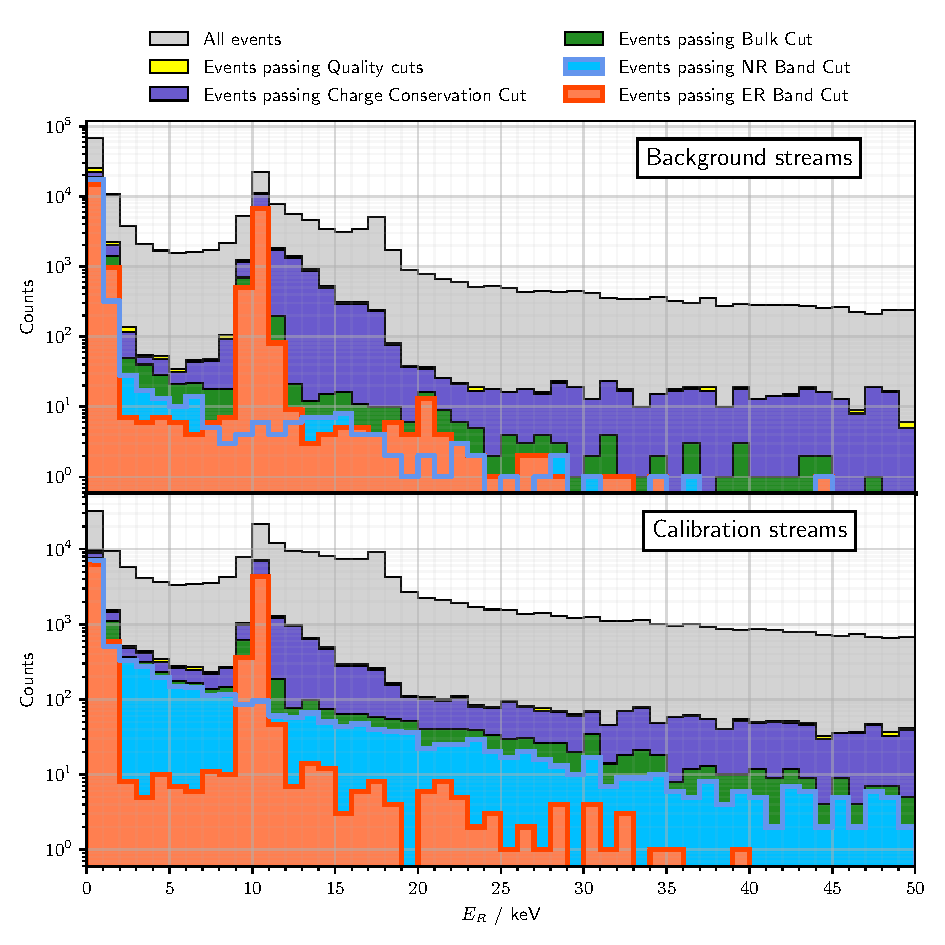
\includegraphics[scale=1]{Figures/Neutron/cut_histogram.pdf}
\caption{Recoil energy $E_R$ Spectra of the events originating from the Background streams (top plot) and the Calibration streams (bottom plots). Each overlapping histogram is associated with an analysis cut. The width of all the bins is \SI{1}{\kilo\eV}.}
\label{fig:cut-histogram}
\end{figure}

The overlapping histograms let us appreciate the amount of discarded events by each analysis cut depending on their recoil energy. We can note some usual features in this histogram like the noise blob at the lowest energies and \SI{10.37}{\kilo\eV} calibration peaks. A visible consequence of the band overlapping at low energy is the attribution of the noise blob events to both the ER and NR band. The contribution of the \SI{1.3}{\kilo\eV} calibration events to the spectra is only perceptible in the second bin of the Background plot.
The comparison of the Background and Calibration energy spectra levels should be made relative to the total number of events. Indeed, the two configurations have different live time calculated in the table \ref{tab:live-time-cut}. Here, we confirm that the Calibration streams, with a cumulative live time of \SI{75.6}{\hour}, recorded more events than the Background streams, with the lower live time of \SI{35.93}{\hour}.
The major difference between the Background and Calibration is the relative levels of the ER band and NR spectra. For the Background configuration, the NR band spectrum has a similar level to the ER band spectrum, excepting the calibration peaks. In the case of the Calibration configuration, the NR band level is an order or two greater than the ER band background spectrum. This is consistent with the higher neutron flux induced by the neutron source.

Until now, the recoil energy was calculated from the heat energy $E_{heat}$ and the bulk ionization energy $E_{Ion.}^{bulk}$ using the equation \ref{eq:er-quenching}. While unbiased, the precision of the recoil energy calculation is limited by the relatively high error on the ionization energy measurement compared to the heat channel.
%, as discussed in section \ref{par:experimental-resolution}.
Now that the events passing the NR and ER band cuts are considered as being generated from nuclear and electronic recoils respectively, it is possible to boost the resolution of the recoil energy $E_R$ using their theoretical quenching factor. For the ER events, the quenching is $Q_{ER}=1$ while for the NR events, the quenching $Q_{NR} (E_R)$ is derived from the Lindhard model in equation \ref{eq:lindhard}. As this quenching is in itself a function of the recoil $E_R$, it is necessary to numerically solve the following equation:
\begin{equation}
\label{eq:er-from-heat}
E_R 
=
E_{Heat} 
\cdot
\frac{
1 + \frac{V_{bias}}{\epsilon_{e^--h^+}}
}{
1 + Q_{NR} \left( E_R \right)\frac{V_{bias}}{\epsilon_{e^--h^+}}
}
\end{equation}
With this calculation of the recoil energy, the ionization measurement is not used. The precision on the estimation of the recoil energy is now only limited by the error of the heat energy measurement.

In order to translate the recoil energy spectrum of the NR band into a measurement of the IP2I neutron background, it is necessary to estimate the nuclear recoil rate rather than their count. Once done, it is possible to compare directly Background and Calibration configurations. This part of the analysis is thoroughly explained in the next section.


\section{Translating the Nuclear Recoil Counts to Rate}

The objective of the analysis presented in the previous section \ref{par:analysis-data-streams} is to count the number of nuclear recoils recorded in the data streams in the Background and Calibration configurations. This eventually resulted in the recoil energy spectra presented in the figure \ref{fig:band-cuts}. In this state, this result do not represent the neutron flux at the IP2I cryostat facility. 
Indeed they consist in an event count which is an extensive quantity depending on the experimental setup and analysis pipeline. The number of recorded events is proportional to the detector exposure, its triggering threshold and the analysis cut efficiencies. The final nuclear recoils count is dependent from the parametrization of the analysis cuts, in particular the tolerance of the analysis cuts. The $2 \cdot \sigma$ tolerance chosen for the analysis cuts yields a selection of well-reconstructed events at the cost of discarding a massive fraction of all the triggering events. 

The neutron flux should be quantified with an intensive quantity which is the event rate. This section explains how the nuclear recoil spectra are translated into nuclear recoil rates. 
Most of the efforts are focused on estimating the actual number of interactions which resulted in a nuclear recoil in the RED80 crystal during the data acquisition. This estimation is described in the next section \ref{par:pulse-simulation} using the technique of pulse simulation.
This is followed by the normalization of the interaction counts described in the section{par:normalization}.


\subsection{Pulse simulation}
\label{par:pulse-simulation}

This section presents the "pulse simulation" technique. It is used to estimate the real number of events that did happen in the RED80 detector from the count of the events passing the band cuts presented in the figure \ref{fig:cut-histogram}. The pulse simulation is used to correct the counts in two ways. 
Firstly, it allows the calculation of the efficiencies associated with the trigger and the data cut. Secondly, it permits the correction of the band contaminations due to the ER, NR and HO bands overlapping at the lowest energies.
The pulse simulation is based on simulating pulses of known recoil energy $E_R$ and quenching $Q$. A pulse designates the signal generated by an event on the five measurement channels being the heat and the ionization $A$ through $D$.

%Although most of these events present a complete charge collection associated with a quenching $Q_{ER}=1$, some are subjects to incomplete charge collection (and still taken into account ??? are discarded ??? idk).

The simulation of a \SI{0.5}{\s} pulse window comes from scaling a pulse template. The heat and ionization signals of the template are the analytical models presented in the section \ref{par:data-format}. The ionization signal is simply modeled by a Heaviside function of the time (eq. \ref{eq:ionization-channel-signal-function}). The heat signal is modeled by the 3-decaying exponential model presented in equation \ref{eq:heat-channel-signal-function} with multiples parameters depending on the thermodynamic properties of the RED80 detector. As explained in the section \ref{par:optimal-filtering}, the parameters are adjusted from the \SI{10.37}{\kilo\eV} calibration events passing the bulk cuts. One should note that due to the non-linearity in the heat response discussed in chapter \ref{ChapterEthem}, the template shape deviates from the pulse shape of measured events at energies higher than \SI{10.37}{\kilo\eV}. This induces a loss of accuracy for the pulse simulation. Therefore, from now on, the analysis is limited to the recoil energy range $[0,\ 50]\ \si{\kilo\eV}$. This limited energy range should pose no threat to the measurement of the neutron background as it is expected to be observed at low energy thanks to kinematics considerations and confirmed by the uncorrected energy spectra associated to the NR band presented in the figure \ref{fig:cut-histogram}.

In order to simulate an event, each channel of the normalized template is scaled to a scaling energy $E_{heat}^{scaling}$ for the heat channel and $E_{X}^{scaling}$ for the ionization channel $A$ through $D$. 
These scaling energies are derived from the heat energy $E_{heat}$ and ionization energy $E_{X}$ from a bank of reference events. These bank of reference events corresponds to the \SI{10.37}{\kilo\eV} calibration events passing the quality cuts. As such, this bank of event should be representative of all the events also featured event with incomplete charge collection. As to facilitate the reading of the scaling energies, the energies of the reference \SI{10.37}{\kilo\eV} calibration events in this reference bank are noted $E_{heat}^{bank}$ and $E_{X}^{bank}$  for the heat and ionization channels respectively.

For this work, the pulse simulation is operated for four different population of events. The most readily available population are the electronic recoils with a recoil energy of $E_R = \SI{10.37}{\kilo\eV}$. As simulated events, they are denominated the \SI{10.37}{\kilo\eV} line and are emulating the \SI{10.37}{\kilo\eV} calibration peak. The scaling energies are simply:
\begin{equation}
\begin{cases}
\displaystyle
E_{heat}^{scaling} = E_{heat}^{ref.}
\\
\displaystyle
E_{X}^{scaling} = E_{X}^{ref.} \quad \textsf{with} \quad X \in \{A,B,C,D\}
\end{cases}
\end{equation}

The second simulated population are the electronic recoils with a recoil energy of $E_R = \SI{1.3}{\kilo\eV}$.  This simulated population is deemed the \SI{1.3}{\kilo\eV} line and is emulating the other calibration peak at \SI{1.3}{\kilo\eV}. The scaling energies are now:
\begin{equation}
\begin{cases}
\displaystyle
E_{heat}^{scaling} = E_{heat}^{ref.} \cdot \frac{1.3}{10.37}
\\
\displaystyle
E_{X}^{scaling} = E_{X}^{ref.} \cdot \frac{1.3}{10.37} \quad \textsf{with} \quad X \in \{A,B,C,D\}
\end{cases}
\end{equation}

The next simulated population corresponds to the electronic recoil band. These simulated events form the so called "flat ER" population. This denomination comes from the uniform distribution $\mathcal{U}(0,50)$ of input recoil energy $E_R^{input}$ on the $[0,\ 50]\ \si{\kilo\eV}$ analysis range of these events.
For each event of the flat ER line, the scaling energies are:
\begin{equation}
\begin{cases}
\displaystyle
E_R^{input} \sim \mathcal{U}(0,50)
\\
\displaystyle
E_{heat}^{scaling} = E_{heat}^{ref.} \cdot \frac{E_R^{input}}{10.37}
\\
\displaystyle
E_{X}^{scaling} = E_{X}^{ref.} \cdot \frac{E_R^{input}}{10.37} \quad \textsf{with} \quad X \in \{A,B,C,D\}
\end{cases}
\end{equation}

The last simulated population corresponds to the nuclear recoil band. This population is denominated the "flat NR" population. As for the previous population, the recoil energy is sampled from the uniform distribution $\mathcal{U}(0,50)$. In order to simulate the characteristics of nuclear recoils presented in the system of equations \ref{eq:nr-band}, the scaling ionization energies are obtained from the quenching factor associated with nuclear recoils $Q_{NR}$ derived from the Lindhard model. To first order, the scaling energies of the events belonging to the flat NR line are:
\begin{equation}
\begin{cases}
\displaystyle 
E_R^{input} \sim \mathcal{U}(0,50)
\\
\displaystyle
E_{heat}^{scaling} = E_{heat}^{ref.} \cdot \frac{E_R^{input}}{10.37}
\\
\displaystyle
E_{X}^{scaling} = E_{X}^{ref.} \cdot \frac{E_R^{input}}{10.37}  \cdot Q_{NR} \left( E_R^{input} \right)
\quad \textsf{with} \quad X \in \{A,B,C,D\}
\end{cases}
\end{equation}

Once the pulses are simulated, they are injected into the experimental data streams. This injection consists in adding the \SI{1}{\s} signal at known randomized time $t_0^{input}$. As such, the pulse simulation technique is only valid when the whole stream of data is saved as described in section \ref{par:data-format}. In order to keep this probing technique from altering too much the characteristics of the analysis, it is decided to inject a maximum of 60 pulses per hour of streams. This process is repeated multiple times with different $t_0$ and for the four simulated population independently. In the end, it is a total of 1 million of each population that are simulated. Just as for the real measured data streams, the newly created streams with injected pulses are processed using the same pre-processing and analysis pipeline.
The figure \ref{fig:band-cut-ecei-simu} presents the simulated events passing the quality and bulk cuts. At the top is the scatter of the bulk ionization energy $E_{Ion.}^{bulk}$ versus the heat energy $E_{heat}$. At the bottom is the graph of the estimated quenching $Q$ and estimated recoil energy $E_R$ of each event. Each simulated population has its own color.

\begin{figure}
\centering
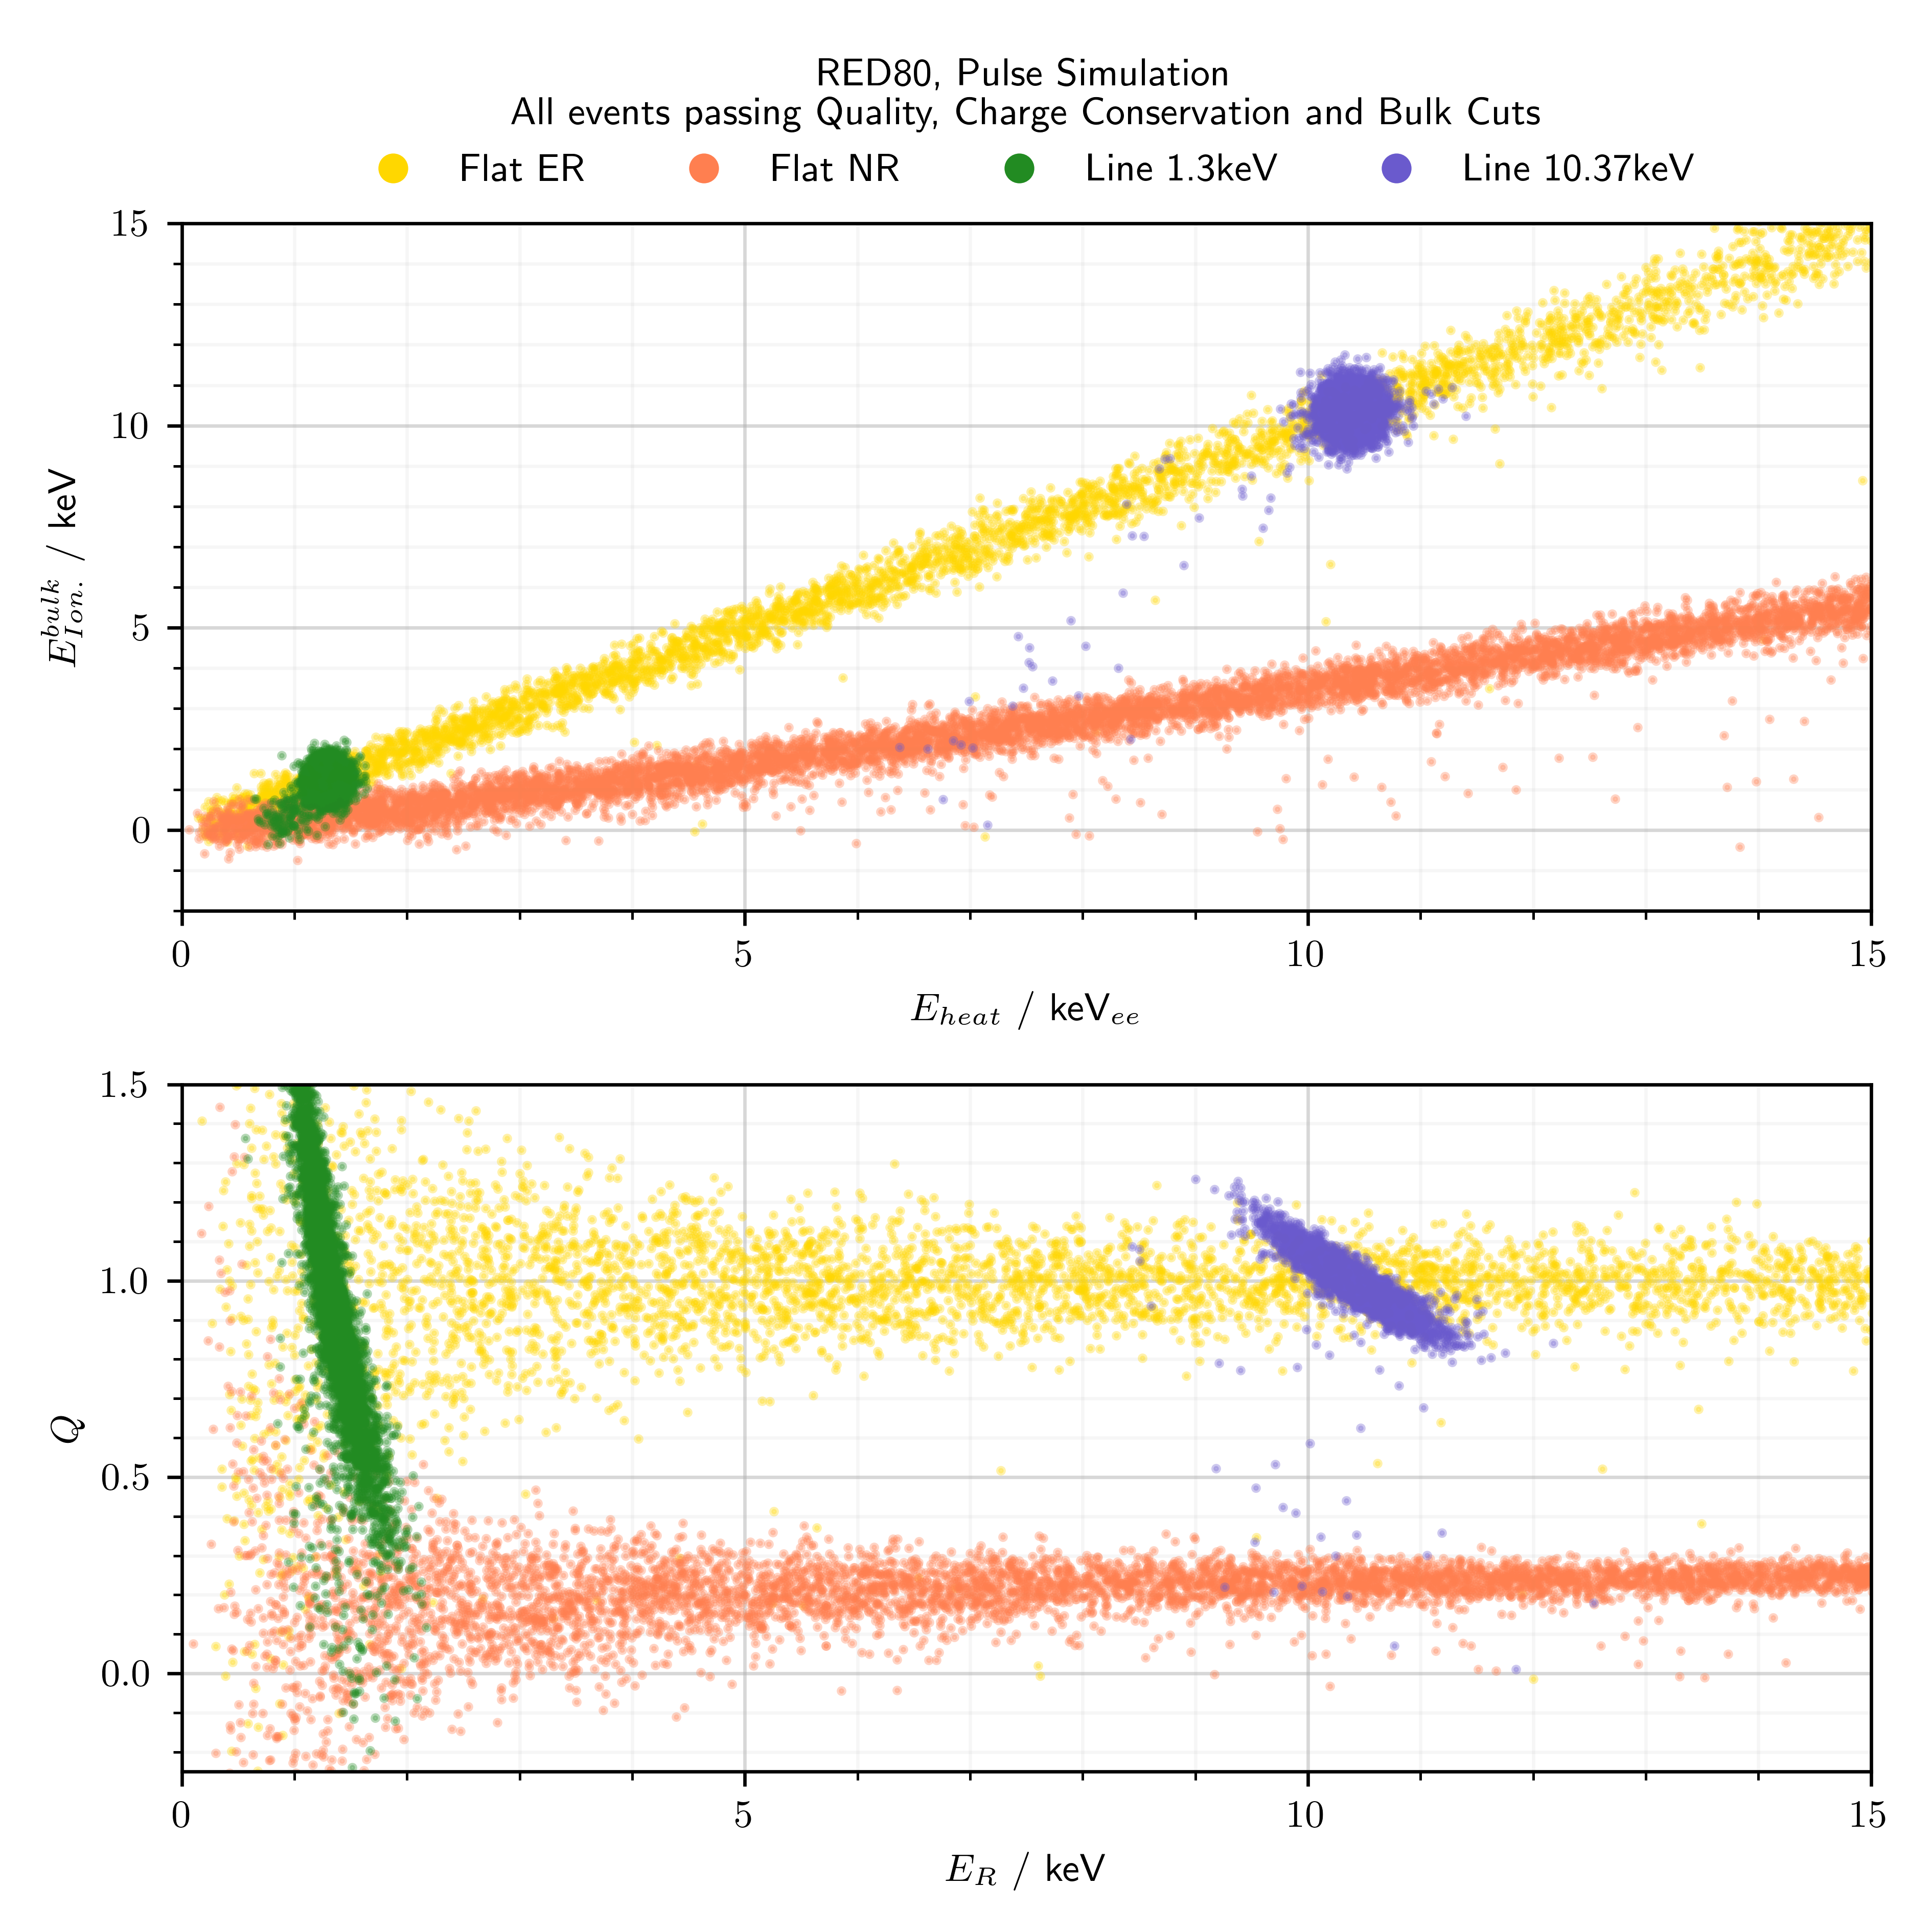
\includegraphics[scale=1]{Figures/Neutron/pulse_simulation.png}
\caption{Illustration of the Pulse Simulation of the four population of events. The top plot represents the bulk ionization energy $E_{Ion.}^{bulk}$ versus the heat energy $E_{heat}$. The bottom plot displays the estimated quenching factor $Q$ versus the estimated recoil energy $E_R$.}
\label{fig:band-cut-ecei-simu}
\end{figure}

These simulated pulses are excellent facsimiles of the real pulses, especially at the lowest energies, with the major advantage that we know their input recoil energy $E_R^{input}$, their injection time $t_0^{input}$ and the type of recoil they emulate. We can thus proceed with the estimation of the efficiency of the pre-processing trigger and the analysis cuts.

%An important remark is to be made here concerning the signal noise injected in the streams along with the simulated pulses. The 10.37keV events composing the bank of events and used for the creation of the simulated population are real events from the streams affected a signal noise. By adding simulated pulses to the streams, we are effectively adding the noise of the simulated pulse and the noise of the stream. This means that all the pulses that are injected into the streams are by construction noisier than real pulses.
%While the effect of this phenomenon is negligible at low energies as the 10.37kev and its associated noise were scaled down, for higher energies this additional noise might result in a worse energy reconstruction than real pulses as well as lead to a discarding by the $\chi^2$ cut.
%As a concrete example, an injected pulse of the "10.37keV line ER" population should be affected by a noise PSD with a factor $\sqrt{2}$ higher than the noise PSD of a real 10.37keV pulses of the stream. This will result in a biased $\chi^2$ value for the simulated pulse, sampled from a $\chi^2$ distribution of mean $\sqrt{2}N$ rather than $\sqrt{N}$. Hopefully, the $\chi^2$ cut of this analysis (presented in \ref{par:quality-cuts}) are large enough to alleviate this effect. As for the energy reconstruction, the bias should be compensated by the energy resolution of the sensors.


\section{Trigger Cut}
\label{par:trigger-cut}

The trigger is a pre-processing step described in section \ref{par:trigger}. Its role is to detect and create the \SI{1}{\s} pulse windows, that is to say triggering event, from a data stream. The objective of this section is to decide whether a simulated event injected at a time $t_0^{input}$ has triggered in the pre-processing. As discussed in section \ref{par:trigger}, there are two conditions necessary to trigger. First, a triggering event shows an amplitude greater than the trigger threshold. And then, triggering events should be spaced in time by no less than \SI{5}{\milli\s} as to avoid the pile-up effect.

In the case of simulated events of known input time $t_0^{input}$, there is a supplementary condition that should be fulfilled for the simulated event to properly trigger. This condition is tied to the difference between the input time and the time reconstructed by the pre-processing process. Its role is to prevent a simulated pulse of low energy which could not have reached the trigger threshold on its own to have trigger by being injected close to an existing experimental pulse of sufficient amplitude energy. This condition is enforced by comparing the input time $t_0^{input}$ of the simulated pulse to the measured time $t_0$ of all the triggering events in the considered stream. A maximum tolerance of \SI{5}{\milli\s} between the injection time  $t_0^{input}$ and the reconstructed time $t_0$ of a simulated pulse. This condition is represented by the inequality:
\begin{equation}
| t_0^{input} - t_0 | \leq 5\textsf{ms}
\end{equation}
Simulated events which triggers in the pre-processing and satisfies this additional condition  are considered as having properly triggered. For the sake of denomination, these events are called "triggering events" having successfully passed the "Trigger cut". 
It is important to note that this trigger cut is specific to simulated pulses.
%and is represented as such in the summary scheme \ref{fig:scheme-ip2i} of the analysis cuts. 

Reproducing this trigger cut with real pulses can only be done if we know the exact time of the energy deposit in the crystal. Access to this piece of information is impossible in this work using either the neutron source or the intrinsic calibration peaks of the germanium as in both cases they follow intrinsically stochastic process of radioactive decay. However, the use of controlled source of particles, such as a controlled pulsing LED or a pulsed neutron source are envisioned.

%Now that we have selected the simulated pulses which properly triggered, the entire analysis chain of this very chapter \ref{ChapterNeutron} described until now is applied to these events. The triggering simulated events population is pruned of the reconstruction biased with the quality cuts and are then allocated to the ER, NR and HO bands (see Figure \ref{fig:band-cut-ecei-simu})


\section{Efficiency correction}
\label{par:efficiency}

The objective of all the analysis cuts is to prune any events with bad energy reconstruction. However, in this process, the majority of the initial experimental events are discarded. This observation is also applicable to the pre-processing trigger. In the end, only a fraction of all the recoils in the germanium crystal do trigger and satisfy the analysis cuts. These remaining are counted and presented as the recoil energy spectra of the neutron background displayed in the figure \ref{fig:cut-histogram}. As to estimate the NR and ER background, it is necessary to estimate the initial number of recoils. This estimation is calculated by correcting the measured counts of NR and ER with the efficiency of the trigger and analysis cuts.

In the presented analysis, a cut is essentially a binary classification. This means that a cut classifies a given set of events into two groups. For example, the quality cut is a test which discriminates the events with evidences of good energy reconstruction from others. However, as all the cuts rely on estimators, the classification on an event by a analysis cut can differ from the actual status of the event. This leads to four possible combinations of the outcome of the cut and the actual condition on the tested event. The table \ref{tab:binary-classification} defines these four combinations.

\begin{table}[]
\centering
\begin{tabular}{cc||c|c}
 &  & \multicolumn{2}{c}{Actual Condition of the Event} \\ \cline{3-4} 
 &  & Condition Positive       & Condition Negative      \\ \hline \hline
\multicolumn{1}{c|}{\multirow{2}{*}{\begin{tabular}[c]{@{}c@{}}Classification\\ of the Event\\ from the Analysis Cut\end{tabular}}} &
  Test outcome positive &
  \begin{tabular}[c]{@{}c@{}}True Positive\\ (TP)\end{tabular} &
  \begin{tabular}[c]{@{}c@{}}False Positive\\ (FP)\end{tabular} \\ \cline{2-4} 
\multicolumn{1}{c|}{} &
  Test outcome negative &
  \begin{tabular}[c]{@{}c@{}}False Negative\\ (FN)\end{tabular} &
  \begin{tabular}[c]{@{}c@{}}True Negative\\ (TN)\end{tabular}
\end{tabular}%
\caption{Table of the four combinations of actual event condition and assigned condition by an analysis cut.}
\label{tab:binary-classification}
\end{table}

The efficiency of a test is defined as the number of true positive events normalized by the number of tested events. However, the efficiency of an analysis cut shows a dependency with the recoil energy $E_R$ and recoil type $RT$ of the tested events. As such, the efficiency $\mathcal{F}$ is defined as a sequence with its $k$th element given by:
\begin{equation}
\mathcal{F}_k
=
\frac{ N_k^{TP} (RT)}{ N_k^{tot} (RT)}
\end{equation}
%=
%\frac{ N_k^{TP} }{ N_k^{TP} + N_k^{FP} + N_k^{FN} + N_k^{TN} }
with $N_k^{TP}$, the number of "True Positive" events in the $k$th bin in recoil energy $E_R$, and $N_k^{tot} = N_k^{TP} + N_k^{FP} + N_k^{FN} + N_k^{TN}$, the total number of events.

These counts of events are estimated with the pulse simulation. Indeed, contrary to the experimental events, the initial number of injected simulated events $N_k^{tot} (RT; simu.)$ is known for each of the recoil type $RT$: nuclear recoil are emulated with the "flat ER" population while the electronic recoils are emulated with the "flat ER" population. Similarly, with the application of the analysis cuts to the simulated events, the counts of true positive events $N_k^{TP} (RT; simu.)$ is measured.

One should note the important difference between the simulated pulses used to estimate the efficiency and the experimental pulses, with their counts corrected by this efficiency. For the experimental pulses, there is no direct access to the number of true positive events, but there rather is count $N_k^{cut} (RT; exp.)$ of all the events passing an analysis $cut$. As the data streams are long, the analysis is not limited by the statistic. Thus, the analysis cuts are parametrized with conservative $2\sigma$ tolerances.  With this parametrization, it is expected to have a very low count of false positive events at the cost of having very high count of false negative. As a result, for this analysis, it is assumed that the count of false positive events is negligible:
\begin{equation}
N_k^{cut} (RT; exp.) = N_k^{TP} (RT; exp.) + N_k^{FP} (RT; exp.) \approx N_k^{TP} (RT; exp.)
\end{equation}
Consequently, the measured count $N_k^{cut} (RT; exp.)$ is an excellent estimator of the number of experimental true positive events $N_k^{TP} (RT; exp.)$.

The efficiency of the analysis cuts $\mathcal{F}$ is therefore estimated from the pulse simulation and used to estimate the initial number of experimental recoils $N_k^{tot} (RT; exp.)$ from the measured counts illustrated by the recoil energy spectra in figure \ref{fig:cut-histogram}. Independently from the binning, the initial number of experimental recoils is calculated in each $k$th bin in recoil energy $E_R$ as:

\begin{equation}
\label{eq:efficiency-correction}
N_k^{tot} (RT; exp.)
=
\mathcal{F}_k (band) \cdot N_k^{bulk} (RT; exp.)
=
\frac{ N_k^{TP, band} (RT; simu)}{ N_k^{tot} (RT; simu)} \cdot N_k^{band} (RT; exp.)
\end{equation}

The figure \ref{fig:cut-efficiency} presents the efficiency $\mathcal{F}$ of each analysis cut for the ER and NR types and the two Background and Calibration configurations. The binning in used is parametrized by the bins edges $b_i$:
\begin{equation}
\label{eq:bins-edges}
\begin{cases}
b_i &= b_{i-1} + 2 \cdot \max \left(\sigma_{E_{heat}}^s(b_i) \right)_{s \in streams}
\\
b_0 &= \SI{0}{\kilo\eV}
\end{cases}
\end{equation}
with $\left(\sigma_{E_{heat}}^s(b_i) \right)_{s \in streams}$ the heat resolution of each streams. With this parametrization of the binning, the width $W_k$ of the $k$th bin is expressed:
\begin{equation}
W_k = b_{k+1} - b_{k}
\end{equation}

\begin{figure}
\centering
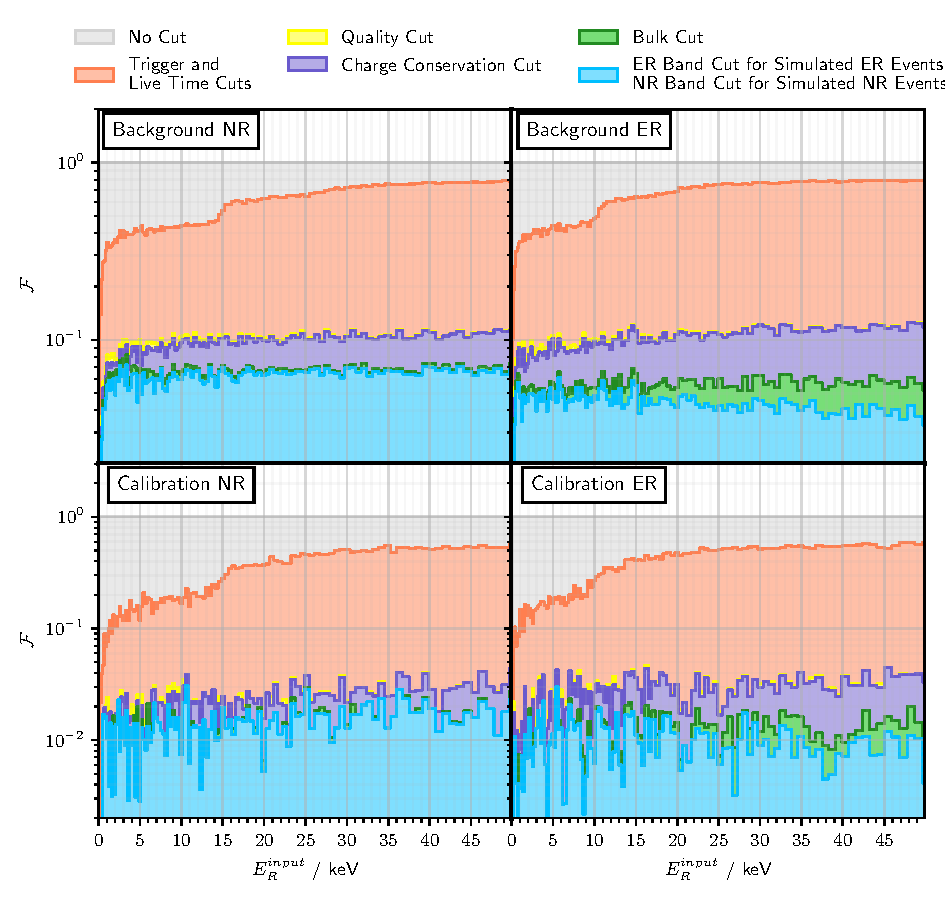
\includegraphics[width=\linewidth,]{Figures/Neutron/cut_efficiency.pdf}
\caption{Efficiency $\mathcal{F}$ of the analysis cuts applied on the simulated events as functions of their input recoil energy $E_R^{input}$. Each subplot corresponds to one of the two Background and Calibration configurations and either the "flat NR" or "flat ER" simulated events. For the "flat NR" events, the NR band cut is drawn. For the "flat ER" events, the ER band cut is displayed.}
\label{fig:cut-efficiency}
\end{figure}

The "No cut" is plotted as a reference cut accepting all the events and has an efficiency of $\mathcal{F}=1$ in each bin by definition. The considered band cut depends on the recoil type of the events: the counts of ER is estimated with the ER band cut while the counts of NR recoils is estimated using the NR band cut.
While the efficiencies associated with all the analysis cuts are plotted, the main efficiency used in the efficiency correction equation \ref{eq:efficiency-correction} is the efficiency of the band cut $\mathcal{F}_k (band)$.

The Background configuration displays higher band cut efficiency $\mathcal{F}_k (band)$ than the Calibration configuration for both the ER and NR. The Background configuration features an efficiency of about \SI{6}{\percent} for the nuclear recoils and about \SI{4}{\percent} for the electronic recoils. For the Calibration, the efficiencies are about \SI{1}{\percent} for the NR events and \SI{0.8}{\percent} for the ER events. This means that this few percent of the initial recoils in the crystal of RED80 induced an event that triggered and passed all the analysis cuts. We can diagnose the successive pruning of the events by studying the efficiency of the previous cuts.

%The efficiency of the trigger cut refines the notion of live time discussed  in the paragraph \ref{par:live-time}. The operating live times $T(Config.)$ are calculated for each $Config.$ in the table \ref{tab:live-time-cut}. These durations implicitly imply that the detector is always available for data acquisition. However, with few tens of percent of discarded events on the whole energy range, the trigger cut prove that the detector has intrinsic tim

% trigger cut
The trigger cut is presented in section \ref{par:trigger-cut}. The efficiency drop of the trigger cut at the lowest energies $\mathcal{O}(\SI{1}{\kilo\eV})$ is explained mainly  by events not reaching the amplitude threshold. However, with few tens of percent of discarded events on the whole energy range, the trigger cut prove that a sufficient amplitude is not enough to triggered upon. Event discarded by the trigger cut can be explained by the screening of the low energy events by events of higher energies. Indeed, the pre-processing parametrization imposes that for events closer than \SI{0.5}{\s}, only the event of higher amplitude is triggered upon. This observation holds on the whole energy range as the trigger cut efficiency is monotonically increasing.
Additionally, one can note the sudden increase in efficiency at about \SI{10}{\kilo\eV} for the ER and \SI{15}{\kilo\eV} for the NR. This feature can be linked to \SI{10.37}{\kilo\eV} calibration peak of the germanium crystal. Indeed,  the crystal of RED80 is neutron-activated resulting in a high rate of \SI{10.37}{\kilo\eV} electronic recoils. These events are screening the events of heat energy $E_{heat} < \SI{10.37}{\kilo\eV}_{ee}$. This heat energy readily corresponds to a recoil energy of $E_R=\SI{10.37}{\kilo\eV}$ for the ER events. For the NR events, the corresponding energy is obtained through the expression of the heat energy $E_{heat}$ as a function of the recoil energy $E_R$ and the quenching $Q_{NR}$ for a nuclear recoil in the equation \ref{eq:nr-band}:
\begin{equation}
\label{eq:15kev-enigma}
E_{heat} = \SI{10.37}{\kilo\eV}_{ee} 
= 
E_R 
\cdot
\frac{
1 + Q_{NR} \left( E_R \right)\frac{V_{bias}}{\epsilon_{e^--h^+}}
}{
1 + \frac{V_{bias}}{\epsilon_{e^--h^+}}
} \cdot E_R
\quad \Rightarrow \quad
E_R = \SI{14.82}{\kilo\eV}
\end{equation}
The Lindhard quenching model is applied to estimate the value of $Q_{NR}$. The equation is numerically resolved, yielding the recoil energy $E_R = \SI{14.82}{\kilo\eV}$. This value is indeed consistent with the energy of the sudden increase in efficiency.

All-in-all, the asymptotic efficiency of the trigger cut is about \SI{80}{\percent} for the Background configuration. This observation is symptomatic from an above-ground experiment with reduced shielding and subject to the natural radioactivity and cosmic rays inducing a relatively high rate of event in the detectors. As for the Calibration configuration, this asymptotic efficiency is even lower \SI{50}{\percent}. Indeed, with the neutron source facing the detector, the event rate is boosted by the intense rate of nuclear recoils.

% Quality cuts
The quality cut, defined in section \ref{par:quality-cuts}, discards the events showing evidence of problematic energy reconstruction. The efficiency drops to approximately \SI{10}{\percent} for the Background configuration and \SI{10}{\percent} for the Calibration configuration. We also note that the increasing step for the trigger cut efficiency caused by the \SI{10.37}{\kilo\eV} calibration events has vanished. This is explained by considering that all the events presenting a pile-up effect (usually with a \SI{10.37}{\kilo\eV} calibration ER event) were discarded by the quality cuts. As the total event rate is higher for the Calibration configuration, the pile-up effect is affecting more events and thus the quality cuts are pruning more than for the Background configuration.

% Charge conservation cut
The charge conservation cut effect seems marginal for both recoil types and the two neutron source configurations. As discussed in section \ref{par:charge-conservation-cut}, there is no concrete evidence of event population not satisfying the electric charge conservation. As such, only events with outlying charge conservation energy $E_{CC}$ are discarded.

%for the NR recoils and the lower-half of the energy range in the case of ER recoils. The slight suppression of the higher-half of the ER recoils spectra could be attributed to a more significant trapping of the electric charges in the crystal (see Chapter \ref{Electrodes}).

% Bulk cut
The bulk cut then comes into play and have a significant effect on all the energy range for each combination of recoil type and configuration. As defined in section \ref{par:bulk-cut}, this cut selects the events not generating a signal on the guard electrodes $A$ and $C$ with inducing recoil in the bulk region of RED80 crystal. As such, the efficiency of the bulk cut should be proportional to the fiducial volume of RED80. This assumption could be verified by running a scan on the voltage bias $V_{bias}$ of RED80, this affecting the fiducial volume as demonstrated in Chapter \ref{ChapterElectrodesScan}, and computing the efficiency for each point.

% Band cut
Finally, the band cut, defined in section \ref{par:band-cut}, seems to discard a negligible fraction of the events. This is to be associated with the figure \ref{fig:band-cuts}: a majority of the events are allocated to either the ER or NR bands, with only a few events kept out.


%We could redraw energy spectra corresponding to this newly estimated number of recoils in the detector. However, the amount of events depends on the exposure of the detector as well as the presented data analysis. Normalization of the histogram is necessary to expressed the measurements independently from the experimental setup and the analysis.


\section{Band Contamination Correction}
\label{par:contamination-correction}

The objective of this section is to correct the counting issue induced by the ER, NR and HO bands overlapping at low energy. This phenomenon is visible on the plots displayed in the figure \ref{fig:band-cuts}. Events in these overlapping areas are attributed to multiple bands and are counted multiple times, hence introducing a significant bias on the recoil energy spectra $N_k^{band} (RT; exp.)$ and the initial number of recoils $N_k^{tot} (RT; exp.)$. With the use of the pulse simulation, it is possible to estimate the contamination rate of the bands into one another.

The most rigorous but resource-intensive method would be to model the distribution of the ER, NR and HO events in term of ionization and heat energy and compute the likelihood function associated to each event. However, given the short time frame induced by the advancement of the \Ricochet{} experiment proposal, it was decided to correct the measurements using quicker binned statistics on the recoil energy spectra. While this latter method effectiveness is heavily affected by the choice of the binning, the induced biases are small and so it constitutes a very good approximation of the more rigorous likelihood method.
%\textbf{ [It also has the advantage of being independent from $dR/dE_R$.] }
 The binning in use for this correction is the same as previously defined from its bin edges in equation \ref{eq:bins-edges}.

This binned analysis is based on the knowledge of the shape of electronic recoil background affecting the detector RED80. Indeed, at the considered energy range, the germanium crystal is only subject to three possible sources of electronic recoils. Two of these sources corresponds to the \SI{1.3}{\kilo\eV} and \SI{10.37}{\kilo\eV} calibration peaks. The other source comes from the Compton scattering processes which is modeled by electronic recoils of uniform distribution in recoil energy, such as the simulated "flat ER" events. It is now possible to produce an empirical model of the recoil energy spectrum created by the electronic recoils. Its value in the $k$th bin for events passing analysis $cut$ is noted $N_k^{cut}(Config.; ER model)$ for the two $Config.$ being Background or Calibration. This model has three empirical components based on the energy spectra of the simulated ER events: the flat ER events $N_k^{cut}(Config.; flat ER)$, the \SI{1.3}{\kilo\eV} line events $N_k^{cut}(Config.; \SI{1.3}{\kilo\eV} line)$ and the \SI{10.37}{\kilo\eV} line events $N_k^{cut}(Config.; \SI{10.37}{\kilo\eV} line)$. Each model components $H_k^{cut}(Config.; simu.)$ is the recoil energy spectrum $N_k^{cut}(Config.; simu.)$ of a simulated population $simu. \in \{flat ER, \SI{1.3}{\kilo\eV} line, \SI{10.37}{\kilo\eV} line \}$ normalized by the total number of simulated events $N_{tot}(simu.)$ of the population. 

The ER background model $N_k^{cut}(Config.; ER model)$  is a linear combination of the three components $H_k^{cut}(Config.; simu.)$. For a configuration $Config.$, in the $k$th bin in recoil energy, the counts of events attributed to the ER background model and passing an analysis $cut$  is expressed as:
\begin{multline}
N_k^{cut}(Config.; ER model)
=
N(Config.; flat ER) \cdot H_k^{cut}(Config.; flat ER) \\
+ N(Config.; \SI{1.3}{\kilo\eV} line) \cdot H_k^{cut}(Config.; \SI{1.3}{\kilo\eV} line) \\
+ N(Config.; \SI{10.37}{\kilo\eV} line) \cdot H_k^{cut}(Config.; \SI{10.37}{\kilo\eV} line)
\end{multline}
with each factor $N(Config.; simu.)$ being a constant. With the chosen normalization of the components, the factors $N(Config.; simu.)$ are interpreted as the initial number of electronic recoils generated by the $simu.$ source, with $flatER$ corresponding to the Compton scattering processes.

%Knowing the amplitude of each components of the electronic background, we also have access the fraction of leakage of each components into the NR and HO bands. Substracting these fraction from the NR and HO band yields corrected energy spectra.

These factors are unknown and are estimated by adjusting the ER background model to the experimental estimation of the ER background. These experimental data consist in the recoil energy spectra $N_k^{ER band}(Config.; exp.)$ of the events passing the ER band cut presented in the figure \ref{fig:cut-histogram}. An issue with this experimental estimation is the overlapping of the ER band cut with the NR and HO band cuts at low energy. This overlapping induces counting of nuclear and heat-only events thus biasing the estimation of the ER background. Moreover, at the lowest energies, the noise blob is passing the ER band cut. This noise blob feature is not taken into account in the ER background model and should not be used for the adjustment. The counter is to consider the events which satisfy only the ER band cut and that are discarded by the NR and HO band cuts. This condition is denominated "ER Band only" and expressed mathematically as:
\begin{equation}
(\textsf{ER Band only}) = ( \textsf{ER Band Cut} ) \textsf{ and not } (\textsf{NR Band Cut}) \textsf{ and not } (\textsf{HO Band Cut})
\end{equation}
The energy spectra formed by the experimental "ER Band only" events does not count the noise blob and has minimal contamination from nuclear recoils and heat-only events.

\sloppy
For each configuration, the ER background model satisfying the "ER Band Only" condition $N_k^{(\textsf{ER Band only})}(Config.; ER model)$ is adjusted to the experimental energy spectra$N_k^{(\textsf{ER Band only})}(Config.; exp.)$ using a minimization of the $\chi^2$ between these functions of the recoil energy $E_R$. The best fitting parameters $N(Config.; simu.)$ are listed in the table \ref{tab:er-background-fitting}.

\begin{table}[]
\centering
\begin{tabular}{cc||c|c|c}
                      &             & \multicolumn{3}{c}{Model Component Factors $N(Config.; simu.)$} \\ \cline{3-5} 
                                                    &            & \begin{tabular}[c]{@{}c@{}}Compton Scattering,\\ Flat ER events\end{tabular} & \SI{1.3}{\kilo\eV} peak  & \SI{10.37}{\kilo\eV} peak   \\ \hline \hline
\multicolumn{1}{c|}{\multirow{2}{*}{Configuration}} & Background & 9808                                                                         & 25289 & 214840 \\ \cline{2-5} 
\multicolumn{1}{c|}{} & Calibration & 65943          & 65158          & 535453        
\end{tabular}%
\caption{Best fitting parameters $N(Config.; simu.)$ for the adjustment of the ER Background model for the neutron source configuration. The graphical representation of the adjustment is presented in figure \ref{fig:neutron-contamination}.}
\label{tab:er-background-fitting}
\end{table}

This adjustment is graphically presented by the left subplots of the figure \ref{fig:neutron-contamination}. The top plots corresponds to the Background configuration while the bottom plots corresponds to the Calibration configuration. Each of the left subplots display the experimental histogram, the adjusted histogram from the ER background model and the three components of this model as illustration. 

\begin{figure}
\centering
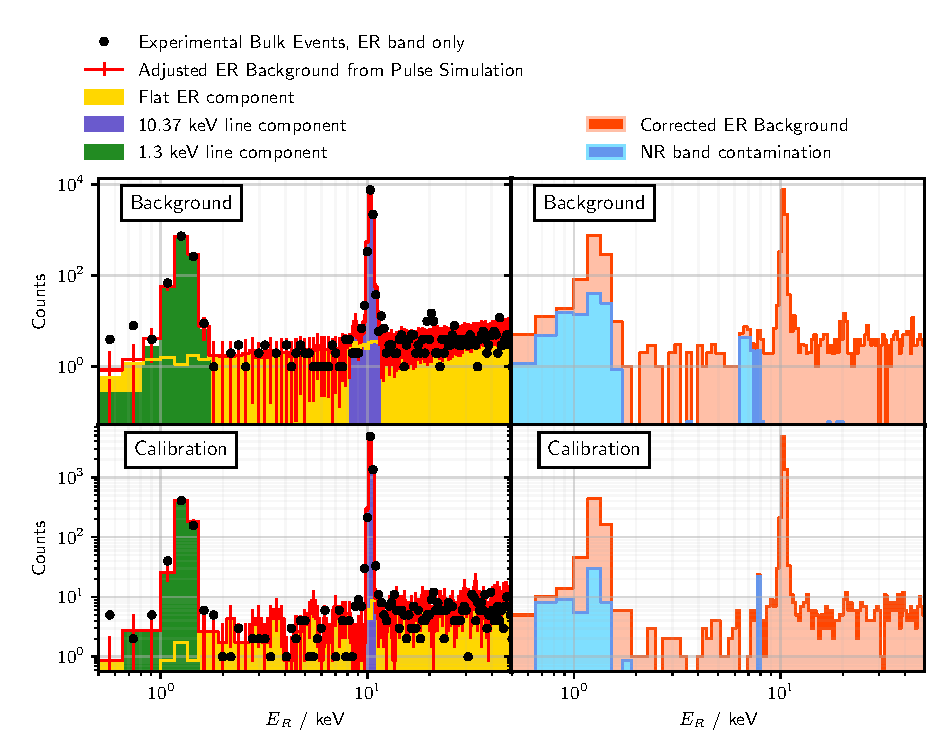
\includegraphics[scale=1]{Figures/Neutron/neutron_contamination.pdf}
\caption{Adjustment of the ER background with the pulse simulation for the Background and Calibration configurations. The left subplots compares the histogram of experimental bulk events passing the ER band cut only with the simulated ER background model and its three components. The best fitting parameters are listed in the table \ref{tab:er-background-fitting}. The right subplots display the counts of ER events contaminating the NR band and the corrected ER background corrected from the contamination. }
\label{fig:neutron-contamination}
\end{figure}

The two right subplots display the two recoil energy spectra. The histograms denominated "NR band contamination" are formed by counting the events from the ER background model which passed the NR band cut $N_k^{\textsf{NR Band}}(\textsf{Config.}; \textsf{ER model})$. As such, it is an estimation of the bias affecting the measurement of recoil energy spectra of the nuclear background presented in the figure \ref{fig:cut-histogram}. 
The terms of the corrected energy spectra associated with the NR and ER are expressed in the $k$th bin as:
\begin{align}
N_k^{\textsf{NR band, corr.}}(\textsf{Config.}; exp.)
&=
N_k^{\textsf{NR band}}(\textsf{Config.}; exp.)
-
N_k^{\textsf{NR Band}}(\textsf{Config.}; \textsf{ER model})
\\
N_k^{\textsf{ER band, corr.}}(\textsf{Config.}; exp.)
&=
N_k^{\textsf{ER band only}}(\textsf{Config.}; exp.)
+
N_k^{\textsf{NR Band}}(\textsf{Config.}; \textsf{ER model})
\end{align}
The correction of the experimental ER Background $N_k^{\textsf{ER band, corr.}}(\textsf{Config.}; exp.)$ is illustrated as the other histogram.

It appears that the contamination of the neutron band occurs mainly near the calibration peaks. The contamination at recoil energy $E_R \approx \SI{8}{\kilo\eV}$ can be explained by \SI{10.37}{\kilo\eV} calibration electronic recoils with incomplete charge collection. The contamination at lower energy range corresponds to some \SI{1.3}{\kilo\eV} event population satisfying the NR band cut. This is consistent with and was expected from the observation of the $Q$ versus $E_R$ plots of figure \ref{fig:band-cuts} for the experimental data and figure \ref{fig:band-cut-ecei-simu} for the pulse simulation.

%It should also be noted that the ER Band is also subject to contamination from nuclear recoils and some heat-only events near the noise blob. As such, the measure and study of the ER background is restricted to the 
%First, we should know what amount of events in each bins of the NR band corresponds to ER recoil. For this, we need to estimate the number of experimental events induced by ER recoil. This estimation is possible because we have a modelization of the ER background. Thanks to the simulated NR events, we know that the NR events leakage into the "Pure gamma" set is negligible. Thus, the set of interest for the ER background modelization fitting is the "Pure gamma" one. The figure \ref{fig:er-components-fitting} presents the histograms of the experimental events for the Background and the Calibration configuration. Each histogram is used to adjust the ER background modelization. 

%We now know the weight, and the number of events,associated to each components of the ER background modelization. Thus, we have now access to the number of simulated events of the 1.3keV, 10.37keV and flat ER population allocated to the NR band. These numbers are therefore substracted from the NR band and added to the ER band. The recoil energy spectrum corresponding to the ER and NR bands are now corrected of cross-contamination for both configuration Background and Calibration.

Following the discussion on the calibration peaks of the germanium presented in the section \ref{par:calibration-sources}, we can actually estimate the electron capture ratio $P_L/P_K$ associated with the \SI{1.3}{\kilo\eV} and \SI{10.37}{\kilo\eV} peaks, from the  and K shells of \ce{^{71}Ge} respectively.
The number of recoils produced by these peaks in the crystal of RED80 is estimated by to the best fitting parameters $N(Config.; simu.)$ presented in the table \ref{tab:er-background-fitting}. The ratios $R_{calib.}(\textsf{Config.})$ between the two peak are:
\begin{align}
\frac{P_L}{P_K}(\textsf{Background}) 
&=
\frac{
N(\textsf{Background}; \textsf{\SI{1.3}{\kilo\eV} line})
}{
N(\textsf{Background}; \textsf{\SI{10.37}{\kilo\eV} line})
}
=
\frac{25289}{214840}
=
0.1177 \pm 0.0008
\\
\frac{P_L}{P_K} (\textsf{Calibration}) 
&=
\frac{
N(\textsf{Calibration}; \textsf{\SI{1.3}{\kilo\eV} line})
}{
N(\textsf{Calibration}; \textsf{\SI{10.37}{\kilo\eV} line})
}
=
\frac{65158}{535453}
=
0.1217 \pm 0.0005
\end{align}
with the $1\sigma$ statistical uncertainty assuming a Poisson statistic for the parameters $N(Config.; simu.)$. The most up-to-date measurement of the electron capture ratio is $P_L/P_K=0.117 \pm 0.001$ \cite{Bambynek:1977}. The difference between this reference value and the two estimation can be explained by systematic uncertainties. As such, the agreement with our measurement is excellent. The replication of this result validates our methodology for the measurement of the electronic and neutron backgrounds.


\section{Normalization of the energy spectra}
\label{par:exposure}
\label{par:normalization}

From experimental data taken with the detector RED80 over a time span of several days, and with a proper processing and analysis of this data, we were able to estimate the number of electronic recoils and nuclear recoils that happened in the detector.
The amount of recoils does depend on the nuclear and electronic background associated with the experimental setup which we want to measure. Yet, it is also proportional to the exposure of the detector as well as the bin width considered for the analysis.

%The bin width $W_k$ was previously discussed in section \ref{par:bin-width} and is used now for this normalization.

The exposure $\mathcal{E}(Config.)$ is expressed in \si{\kg \day}. Its roles is to normalize the event counts in respect to the live time $T_{live}$ and the mass $m_{Ge} = \SI{0.038}{\kg}$ of the RED80 detector:
\begin{equation}
\label{eq:exposure}
\mathcal{E}(Config.) = T_{live} (Config.) \cdot m_{Ge}
\end{equation}
The live time $T_{live}$ corresponds to the duration during which the detector is correctly operating and recording data. For both the Background and the Calibration configurations, the live times are calculated in the table \ref{tab:live-time-cut}.

%{\color{red}Just accept a mass of 38g, measured by the entreprise mirion, maybe add some precision with uncertainty if necessary. Because what i am tryig to discuss here is already taken into account in the fiducial cut paragraph}
%The same concern can be expressed concerning the mass of the detector: by definition the crystal is the only part of the detector used as absorber and contribute to the exposure of the detector. If we want to be even more rigorous, we could say that some fraction of the crystal would not contribute to the exposure. For example, it is known that event happening on the surface of the crystal are subject to edge effects which alter the signal induced by a recoil, discarding it from the analysis through the quality cuts or the charge conservation. Nevertheless, as these surface are entirely negligible, we can consider the mass of the detector to be the mass of the germanium crystal: $m_{Ge} = 38 \textsf{g} = 0.038 \textsf{kg} $.

The presentation of the measurement of the neutron and electronic backgrounds is done with the daily event rate $\mathcal{R}$. This quantity is expressed in \si{events \per \kg \per \kilo\eV \per \day}. Its value in the $k$th energy bin for the configuration $Config. \in \{ \textsf{Background}, \textsf{Calibration} \}$ and the recoil type $RT \in \{ ER, NR\}$ is expressed as:
\begin{align}
\mathcal{R}_k(Config., RT) 
&=
\frac{ N_k^{tot} (Config., RT; exp.) }{ \mathcal{E} (Config.) \cdot W_k}
\\
&=
\frac{ \mathcal{F}_k \cdot N_k^{band} (Config., RT; exp.) }{ m_{Ge} \cdot T_{live}(Config.) \cdot W_k}
\end{align}
using the efficiency correction equation \ref{eq:efficiency-correction}, the detector exposure in equation \ref{eq:exposure}
and the bin width $W_k$ expressed in equation \ref{eq:bins-edges};

The figure \ref{fig:background-measurements} presents the NR and ER backgrounds for the two neutron source configurations as daily event rate $\mathcal{R}_k(Config., RT)$. The main results of this section concern the estimation of the NR backgrounds. We see that the NR event rate of the Calibration is about 50 times higher than for the Background configuration. The reference value is the NR event rate level at the lowest energies, which is about \SI{1e6}{events \per \kg \per \kilo\eV \per \day} for the Calibration and \num{1e4} for the Background. This is consistent with the presence of the neutron source facing the detector RED80 inducing a high neutron flux in the cryostat and creating a heightened nuclear recoil rate. 

\begin{figure}
\centering
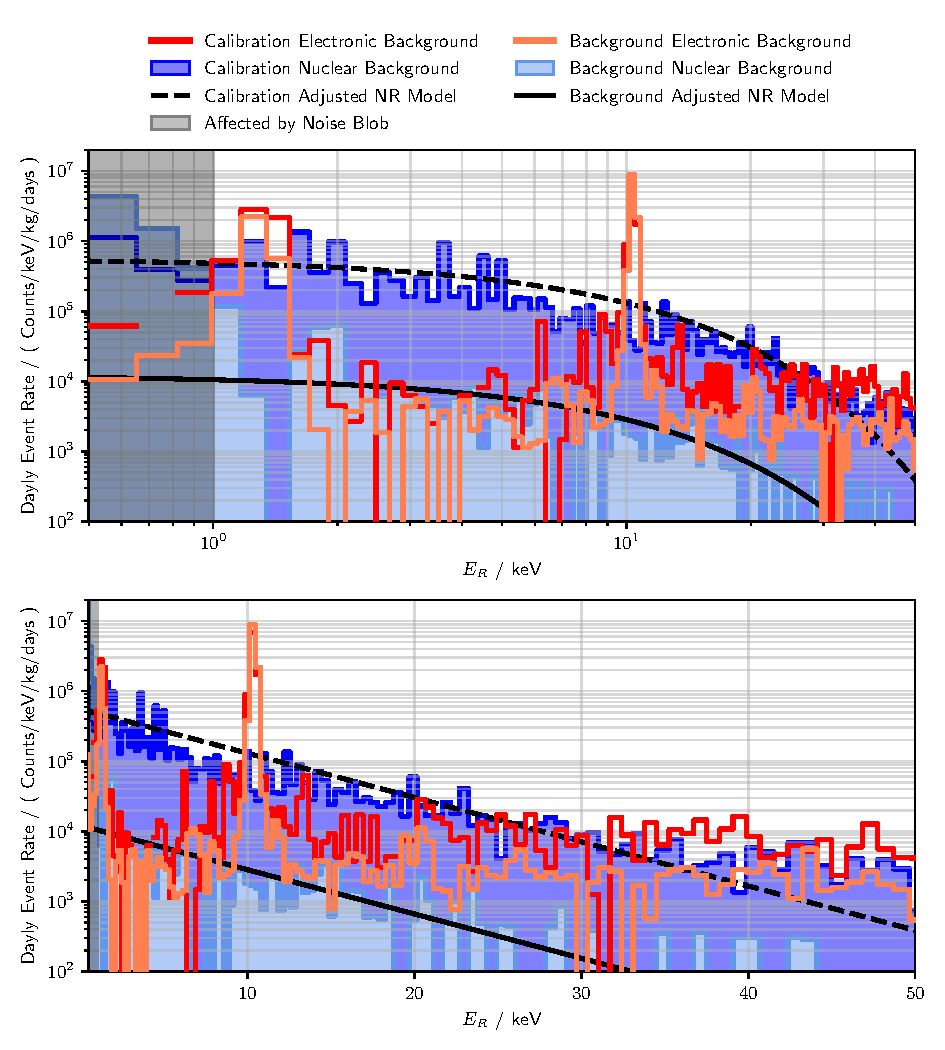
\includegraphics[scale=1]{Figures/Neutron/neutron_background.pdf}
\caption{Neutron and electronic recoil backgrounds expressed as daily event rate $\mathcal{R}_k(Config., RT)$ for the Background and Calibration configurations. Both plots displays the same curves with a logarithmic energy scale on top and a linear energy scale at the bottom. The shaded energy range for $E_R< \SI{1}{\kilo\eV}$ is discarded from integration as being affected by the noise blob.}
\label{fig:background-measurements}
\end{figure}

Both measured neutron backgrounds are adjusted with a background model derived from the kinematic recoil properties. The daily event rate histograms are modeled with the functions:
\begin{align}
\mathcal{R}_k(\textsf{Background, NR model}) &= \mathcal{R}_0(\textsf{Background}) \cdot \exp
 \left( - \frac{ (b_{k+1} + b_{k}) }{2 \cdot E_{cap}} \right)
 \\
\mathcal{R}_k(\textsf{Calibration, NR model}) &= \mathcal{R}_0(\textsf{Calibration}) \cdot \exp 
 \left( - \frac{ (b_{k+1} + b_{k}) }{2 \cdot E_{cap}} \right)
\end{align}
with the expression $(b_{k+1} - b_{k})/2$ corresponding to the center of the $k$th bin in recoil energy. This model of the NR background is parametrized with the three unknown $\mathcal{R}_0(\textsf{Background})$, $\mathcal{R}_0(\textsf{Calibration})$ and $E_{cap}$. The model is adjusted to the experimental NR backgrounds with $\chi^2$ minimization considering a Poisson error on each points. The best fitting parameters are:
\begin{equation}
\begin{cases}
\mathcal{R}_0(\textsf{Background}) &= \SI{1.22e4}{events \per \kg \per \kilo\eV \per \day}
\\
\mathcal{R}_0(\textsf{Calibration}) &= \SI{5.58e5}{events \per \kg \per \kilo\eV \per \day}
\\
E_{cap} &= \SI{6.88}{\kilo\eV}
\end{cases}
\end{equation} 
Both event rates distributions seems to corresponds to the kinematic recoil distribution expected from \si{\mega\eV}-scale fast neutrons.


The ER backgrounds are plotted for illustration and crosscheck. Indeed, we see that the amplitude of the calibration peaks is approximately the same for both configurations. This means that the rate of two calibration electronic recoil peaks is the same between the Background and Calibration configuration. As such, it confirms that the entire analysis processed the Background and the Calibration streams similarly. 

We can note that the flat Compton background is globally higher for the Calibration compared to the Background. This can be explained by the higher neutron flux which produces gamma rays by interacting with the lead shield of the cryostat, and the gammas emitted by the AmBe source.

Comparing the nuclear recoil background and the electronic recoil background, we see that the NR background is predominant over the Compton background from $\mathcal{O}(\SI{10}{\kilo\eV)}$ in the Background configuration. This means that at higher energies, the main component of the energy spectrum is the Compton background, which is typically observed in the past Direct Dark Matter searches. However, the neutron background is becoming the main component of the energy spectrum at lower energy. This means that by improving their energy resolution, the Direct Dark Matter experiments should now be prepared for this new NR background and adapt their shielding. 


\section{Measurement of the ILL neutron background}
\label{par:ill-neutron-background}

The neutron background measurements at the IP2I cryostat with the RED80 germanium detector are used to extrapolate the neutron background that will affect the CryoCube array of germanium detectors in the \Ricochet{} cryostat next to the nuclear reactor of the ILL. The observation of the measured neutron and ER background in figure \ref{fig:background-measurements} confirms that neutron is the most detrimental  for the measure of the CENNS done at low energy. As such, an estimation of this neutron background at the ILL site is vital for the \Ricochet{} experiment.

While the neutron background was measured at the ILL with helium tube detectors with multiple nuclear reactor activities, this technology is only sensitive to energies higher than $\mathcal{O}(\SI{100}{\kilo\eV})$. A way to link the neutron background at high energy with the neutron background at low energy is to measure the same neutron background with the two technologies of detectors. This reference neutron background measurement is made at the IP2I cryostat facility with RED80 and is displayed in the figure \ref{fig:background-measurements}. Measurements at high energies were taken with the helium tube detector in place of the cryostat, with the two same position of the neutron source, leading to the two Calibration and Background configuration. The comparison of the high and low energy spectra should be relative between the Calibration and the Background configurations. For this, we use the nuclear recoil event rate of both configurations integrated over an energy span. The ratio $\mathcal{R}_{Ge}$ of the integration in the interval $[1-50]\ \si{\kilo\eV}$ of the nuclear recoil energy spectra in Calibration and Background is:
\begin{equation}
\begin{cases}
\displaystyle k_0 = \min \left\lbrace k; b_k \leq \SI{1}{\kilo\eV} \right\rbrace
\\
\displaystyle K = \max \left\lbrace k; b_{k+1} \leq \SI{50}{\kilo\eV} \right\rbrace
\\
\displaystyle \mathcal{R}_{Ge}^{exp.} = 
\sum_{k=k_0}^K 
\frac{
\mathcal{R}_k(\textsf{Calibration, NR background}) 
}{
\mathcal{R}_k(\textsf{Background, NR background}) 
}
=
\frac{ 2897511 }{ 79546 }
= 36.4 \pm 0.2
\end{cases}
\end{equation}
with $b_k$ the left bin edge of the $k$th bin as defined in the system of equations \ref{eq:bins-edges}, and calculating the $1\sigma$ statistical uncertainty assuming a Poisson statistic for each integrated rate. As the systematic uncertainties are not considered, the error on the ratio $\mathcal{R}_{Ge}^{exp.}$ is underestimated.
In comparison, the ratio obtained by the helium tube detectors were:
\begin{equation}
\begin{array}{cc}
\mathcal{R}_{Dubna 3-He} &= 26.5 \pm 4.8 \\
\mathcal{R}_{Grenoble 3-He} &= 34.5 \pm 0.5
\end{array}
\end{equation}

As such, the fast background measurement between the cryogenic detector RED80 and the \ce{^3He} detector are compatible with the measurement at high energies. 
%This confirms that estimating the future \Ricochet{} fast neutron background at ILL is possible by operating \ce{^3He} detectors in spectroscopic mode there.
The STEREO experiment located at the future \Ricochet{} site has been removed in December 2020, hence opening the possibility to accurately estimate the expected fast neutron background in \Ricochet{} with the same \ce{^3He} detectors.



%We can also calculate this ratio with the neutron background models adjusted in the previous paragraph. In this case, no integration is needed as the models of the NR background for the Background and Calibration configurations are proportional with a factor:
%\begin{equation}
%\mathcal{R}_{Ge}^{model} = \frac{\mathcal{R}_0(\textsf{Calibration})}{\mathcal{R}_0(\textsf{Background})} = 45.74
%\end{equation}




%%% EXILE LANDS %%%

%
%\begin{equation}
%E_R
%= E_{kin}^N \frac{ 4 m_N m_{Ge} }{ \left( m_N + m_{Ge} \right)^2 } \cos^2(\theta)
%\approx E_{kin}^N \frac{ 4 m_N }{ m_{Ge} } \cos^2(\theta)
%\approx \frac{4}{73} E_{kin}^N \cos^2(\theta)
%\approx \frac{1}{20} E_{kin}^N \cos^2(\theta)
%\end{equation}
%This equation means that a neutron with a kinematic energy of $E_{kin}^N = 200$keV can produces at most a nuclear recoil of energy $E_R = 10$keV.


%\section{Study of the Heat-Only events}
%
%{\color{red} Work ongoing, Coming soon! free DLC}
%The Heat-only events can be induced by several known process:
%\begin{itemize}
%	\item recoil in the NTD passing the Quality cuts (usually at the lowest energy)
%	\item event with a quenching factor $Q=0$ induced by a surface electronic recoil (usually a electron from a $\beta$ decay)
%\end{itemize}
%However, these processes alone can not explain the observations. Some ideas:
%\begin{itemize}
%	\item crystal cracks
%	\item release of energy stocked by inelastic nuclear recoil in the crystal lattice
%	\item ???
%\end{itemize}
%
%\section{Rejection and Leakage}

